%-----------------------------------------------------------------------
%                          hires2_correction.tex
% A&A LaTeX class (aa.cls)
%-----------------------------------------------------------------------
%\documentclass[referee]{aa}    % for a referee version
\documentclass{aa}
\usepackage{graphicx}
\usepackage{txfonts}
\usepackage{placeins}
\usepackage{natbib}
\usepackage[colorlinks,allcolors=blue,bookmarks=false]{hyperref}
\usepackage{xcolor}
\usepackage{amsmath}
\hyphenation{get-sources get-filaments get-images non-uniform back-ground}

\newcommand{\draftnote}[1]{\textcolor{magenta}{\textbf{[#1]}}}
\newcommand{\chg}[1]{\textcolor{magenta}{#1}}
\DeclareRobustCommand{\add}[1]{{\color{green!50!black}#1}}   % new or rewritten text
\DeclareRobustCommand{\del}[1]{{\color{magenta}#1}}          % text to remove
\newcommand{\mH}{m_{\rm H}}
\newcommand{\muH}{\mu_{\rm H_2}}
\newcommand{{\um}}{\,$\mu$m}
\newcommand{\Teff}{T_{\rm F}}
\newcommand{\Dimc}{\mathcal{D}_{\rm C}}
\newcommand{\Dim}{\mathcal{D}}
%%\newcommand{\Sig}{\Sigma}

\begin{document}

\title{Correcting the temperature bias of dust surface density images\\of molecular clouds}

\author{Alexander Men'shchikov\inst{1}}
\institute{D\'epartement d'Astrophysique (DAp), IRFU, CEA Saclay,
Universit\'e Paris-Saclay, 91191 Gif-sur-Yvette, France}

\date{Received / Accepted}
\offprints{Alexander Men'shchikov}
\titlerunning{Correcting the temperature bias of surface density images}

%%%%% -----------------------------------------------------------------------------------------------------------------------------
%%%%% NUMBERS (2026-10-20): the values of the abstract are copied from Sects. 3.2, 5 and 6; see the comments there.
%%%%% -----------------------------------------------------------------------------------------------------------------------------
\abstract{Surface densities of molecular clouds are derived by fitting one modified blackbody to each pixel of far-infrared images.
In dense structures, the fit is dominated by the warmer material along the line of sight and underestimates the surface densities
by more than a factor of two in the densest material. The observed spectral shapes cannot reveal this underestimation, because its
signature corresponds to only a few percent of intensities. This paper presents a correction method for surface densities $\Sigma$,
calibrated on radiative transfer models. The dust temperature $T$ depends only on the effective attenuating column $\Sigma_{\rm A}$
that shields the dust from the interstellar radiation field. A single relation $T(\Sigma_{\rm A})$ describes $2086$ embedded models
of Bonnor--Ebert spheres and $7$ cylindrical filaments with a scatter of $2.4$\%. The correction factor is an explicit function of
$\Sigma$ alone and only slightly depends on the shapes of structures. The method applies to any conventional image of surface
density, obtained with any angular resolution. The method was tested on additional $1815$ models of cores, on isolated filaments,
and on a simulated sky built from radiative transfer models. The correction raises the median core mass from $0.63$ to $0.98$ of
the true mass, the linear densities of filaments from $0.60$--$0.96$ to $0.93$--$1.01$, and the total $\Sigma$ of the simulated sky
to $0.96$. The correction includes dependence on a wide range of strengths $G_{0}$ of the interstellar radiation field, measured on
$9$ supplementary grids of models. Applied to the molecular cloud in Aquila, the correction raises the total $\Sigma$ by a factor
of $1.86$. For the adopted dust properties, the total uncertainties of corrected surface densities are ${\sim}30$\% in diffuse
material and ${\sim}50$\% in dense structures, and those of corrected temperatures ${\sim}2$\,K.}

\keywords{ISM: clouds -- ISM: structure -- Stars: formation -- Infrared: ISM -- Submillimeter: ISM -- Techniques: image processing}

\maketitle
\nolinenumbers

% =====================================================================

\section{Introduction}
\label{sec:intro}

Far-infrared and submillimeter imaging surveys of the nearby and distant molecular clouds with the \emph{Herschel} Space
Observatory \citep{Pilbratt_etal2010} have provided most of the current knowledge about the structures in star-forming regions
\citep[e.g.,][]{Andre+2010, Motte+2010, Andre+2014}. One of the most important quantities is the surface density $\Sigma$ of dusty
gas, derived by fitting an optically thin modified blackbody to the intensities $I_{\lambda}$ of each pixel \citep{Hildebrand1983}.
The fitting gives one dust temperature $T$ and one surface density $\Sigma$ for each line of sight.

Dense cores and filaments are extracted from such images, and every quantity derived from them inherits their accuracy.
Conventional surface density images have a poor angular resolution of $36.3{\arcsec}$ of the longest waveband at $500${\um}. A
multi-resolution differential scheme \citep{Palmeirim+2013} can enhance the resolution to $18.2{\arcsec}$. This work employs the
improved \emph{hires} method \citep{Menshchikov2021method} that produces sharper surface density images at the resolutions of all
observed wavebands. The bias discussed below affects both the conventional and high-resolution images in the same way, because they
are based on the same method of fitting pixel intensities.

A weak point of the fitting procedure is the assumption of a constant temperature. Although it is accurate for diffuse material,
whose temperatures change little along the line of sight, the assumption fails for a cold dense structure embedded in a warmer
cloud. The derived temperature is weighted by the emission, hence by the warmer material, which leads to the underestimated surface
densities. The size of the effect on surface density follows from the sensitivity of the Planck function to the temperature,
\begin{equation}
   \frac{\partial \ln \Sigma}{\partial \ln T} = -\,\frac{x_\lambda}{1-{\exp\left(-x_\lambda\right)}}, \quad
   x_\lambda \equiv \frac{h_{\rm P} c}{\lambda k_{\rm B} T},
\label{eq:sensitivity}
\end{equation}
where $\lambda$ is the wavelength, $c$ is the speed of light, $h_{\rm P}$ is the Planck constant, and $k_{\rm B}$ is the Boltzmann
constant. At $T = 10$\,K, this derivative equals $-9.0$, $-5.8$, $-4.2$, and $-3.1$ at $160$, $250$, $350$, and $500${\um},
respectively. If a cold core's temperature is overestimated by only $1$\,K, the surface density derived at $500${\um} is too low by
$24$\% and the one derived at $160${\um} is underestimated by a factor of $2.3$.

The bias cannot be absorbed into the assumed dust opacity, because it is not a constant factor. It grows with the surface density
of the surrounding cloud, because denser clouds produce larger temperature contrasts along the line of sight, that is, larger
ratios of the temperatures of the warmest and the coldest dust on it. The bias also grows with the concentration of a structure,
because a more concentrated core is better shielded. Two structures with the same true $\Sigma$ in different environments are
therefore recovered with different derived values.

The bias has been studied with radiative transfer models of clouds, cores, and filaments \citep{Shetty+2009b, Malinen+2011,
Juvela+Ysard2012, Juvela+2013}. These studies found that single-temperature fits underestimate the surface density toward the
densest structures, by up to a factor of $3$ \citep{Juvela+2013}. Several ways to recover the temperature structure were proposed.
The observed profiles of a core can be inverted under the assumption of spherical symmetry \citep{Roy+2014}. The emission of each
line of sight can be described by several temperature components and fitted in many wavebands at once \citep{Marsh+2015}. Radiative
transfer models can be fitted to the observed images of a whole field \citep{Juvela+2013}, and empirical models can be used to
combine the wavebands of different resolutions \citep{Juvela+Montillaud2013}. These methods need either an assumed geometry of a
particular structure or a model of the whole field, whereas the correction presented here needs neither. It is calibrated once on
radiative transfer models and then applied to any surface density image, with a factor that depends only on the value of each pixel.

Section~\ref{sec:models} describes the radiative transfer models used to calibrate and test the correction. Section~\ref{sec:law}
derives from the models the relation between the dust temperature and the column that shields the dust. Section~\ref{sec:corr}
turns this relation into the correction. Section~\ref{sec:valid} tests the correction on independent radiative transfer models and
on a simulated sky. Section~\ref{sec:aquila} applies it to the Aquila cloud observed with \emph{Herschel}. The appendices describe
the radiative transfer models, the effects of the arrangement of material along the line of sight, and the calibration for
different radiation fields. They also show why the observed colors and temperatures cannot improve the correction and give the
uncertainties of the corrected surface densities, masses, and temperatures.

In this paper, images are denoted by calligraphic letters, e.g., $\Dim$ for a surface density image and $\mathcal{F}$ for an image
of correction factors. The surface density of a single pixel or line of sight is denoted $\Sigma$; it is the number of hydrogen
molecules per unit area, in cm$^{-2}$. The angular resolution of an image, the full width at half maximum of its beam, is denoted
$O$, and a subscript of an image or of a factor gives $O$ in arcseconds, e.g., $\Dim_{13.5}$ for a surface density image at
$O = 13.5{\arcsec}$.

% =====================================================================

\section{Radiative transfer models}
\label{sec:models}

The surface density correction method is based on accurate radiative transfer models of spherical cores, cylindrical filaments, and
a diffuse cloud, in which the true surface density is known. All models were computed with the Monte Carlo dust continuum
radiative-transfer code \emph{radmc-3d}\footnote{\url{http://www.ita.uni-heidelberg.de/~dullemond/software/radmc-3d}}
\citep{Dullemond+2012} to obtain their one-, two-, or three-dimensional dust temperature structure and images of their surface
density and emergent surface brightness in the \emph{Herschel} photometric bands ($70$, $100$, $160$, $250$, $350$, and
$500$\,$\mu$m).

The models were heated from outside by the isotropic interstellar radiation field \citep{Black1994}, of strength $G_0=0.98$ in
\citet{Habing1968} units, to which a hot blackbody component of $2.2{\times}10^4$\,K was added to obtain stronger fields.
Integrated over its far-ultraviolet part, the adopted fiducial field has $G_0 \approx 10$. The dust opacity was that tabulated by
\citet{Ossenkopf+Henning1994} for grains with thin ice mantles, corresponding to coagulation time of $10^{5}$\,yr and hydrogen atom
number density of $10^{6}$\,cm$^{-3}$. The opacities were scaled by a factor of $1.0746$ to match the analytic approximation
$\kappa_\lambda = 10\,(300\,\mu{\rm m}/\lambda)^2\,{\rm cm^2\,g^{-1}}$ commonly used in observational studies. The adopted fiducial
distance of $260$\,pc corresponds to the value previously used for the Aquila cloud \citep{Konyves+2015}. Details are given in
Appendices~\ref{sec:grid} and \ref{app:rtmodels}.

\subsection{Cores}
\label{sec:modcores}

Each model of a core adopted a radial volume density distribution $\rho(r)$ of an isothermal Bonnor--Ebert sphere \citep{Ebert1955,
Bonnor1956} embedded in a uniform spherical cloud. Three grids were computed (Appendix~\ref{sec:grid}). The $2089$ models of the
main grid spanned surface densities of the embedding cloud from $3.75{\times}10^{20}$ to $9.6{\times}10^{22}$\,cm$^{-2}$, masses of
the sphere from $1.6{\times}10^{-3}$ to $31\,M_{\odot}$, and half-maximum widths of its volume density profile from $0.003$ to
$0.25$\,pc, with central-to-edge density ratios from $1.04$ to $2.1{\times}10^{3}$. Three models were optically thick in the far
infrared and were not used. The relation of Sect.~\ref{sec:relation} was fitted to the other $2086$ models and to the filaments.
The $1815$ models of a subdivision grid, with parameters between those of the main grid, served to test the correction
(Sect.~\ref{sec:valgrid}). A grid of radiation fields repeated $339$ models of the main grid in $9$ fields, from $G_0 = 0.98$ to
$483$ (Sect.~\ref{sec:g0corr}).

%The main grid contained 2089 models, spanning wide ranges of the surface
%densities of the embedding cloud, the core sizes, and their central-to-edge volume density ratios. Three models reached the highest
%surface densities and were optically thick in the far infrared.

\subsection{Filaments}
\label{sec:modfil}

Each filament was computed twice, for two purposes. As an isolated cylinder, without any surrounding cloud, it was used to
determine the temperature relation (Sect.~\ref{sec:relation}). Inside a cylindrical envelope that stood for the surrounding cloud,
which shields the outer parts of the filament and makes them colder, it was used to populate the simulated sky
(Sect.~\ref{sec:modcloud} and Appendix~\ref{app:embfil}). The isolated cylinder, $7.2$\,pc long, had the radial volume density
profile
\begin{equation}
  \rho(r) = \rho_{\rm C}\left(1 + \left(2^{2/p}-1\right)\left(\frac{2r}{h}\right)^{2}\right)^{-p/2},
\label{eq:fdens}
\end{equation}
truncated at the radius $R = 0.5$\,pc, where $h$ is the half-maximum width of the volume density profile and the factor
$(2^{2/p}-1)$ makes $h$ independent of the slope $p$ \citep{Menshchikov2021method}. The surface density profile of the cylinder has
the half-maximum width $H\approx 2h$ for the slopes $p = 2$ and $1.75$ of the models. Only the middle section of
each cylinder was used, where the radiation entering through its ends is negligible and the temperature depends only on the
distance $r$ from the axis. The parameters of the eight filaments are given in Table~\ref{tab:cylpar}. The densest one had an
optical depth of $0.84$ at $100${\um} through its axis and was not used, like the three optically thick cores.

\begin{figure*}
\centering
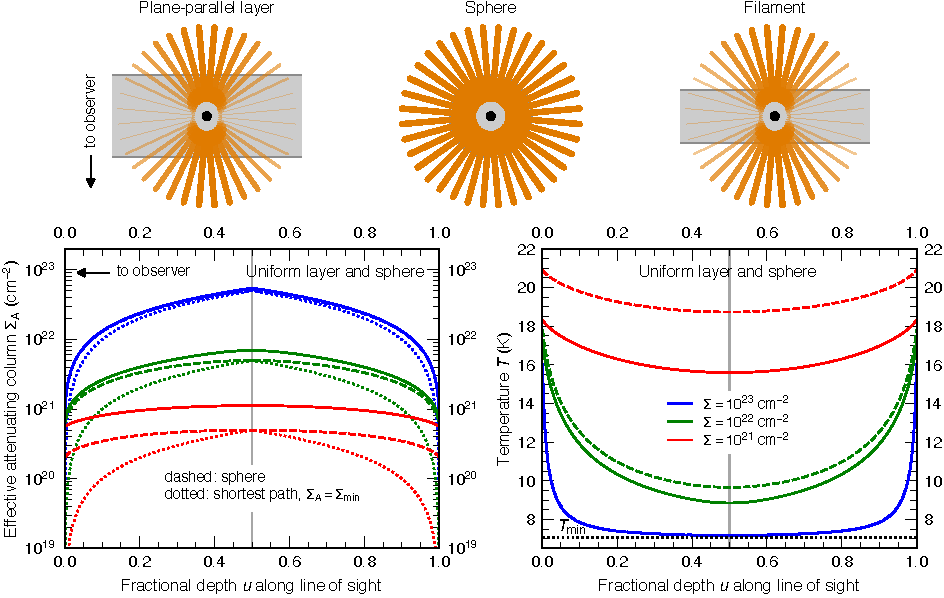
\includegraphics[width=0.85\linewidth]{fig_geometry.pdf}
\caption{Geometry of the dust attenuation in different structures. \emph{Upper}: The radiation that heats a dust grain, marked by
the black point, arrives from every direction having crossed columns of very different lengths. The rays are drawn thicker where
less material has been crossed. Most energy arrives along the normal in the midplane of a layer; no direction is favored at the
center of a sphere; a cylindrical filament has intermediate properties -- resembling a layer along its axis and a sphere across the
axis. \emph{Lower left}: The effective attenuating column $\Sigma_{\rm A}$ of Eq.~(\ref{eq:seff}) against the fractional depth $u$
along the line of sight normal to a uniform-density layer (solid curves) and along the diameter of a uniform-density sphere (dashed
curves), for total surface densities $\Sigma$ of $10^{21}$, $10^{22}$ and $10^{23}$\,cm$^{-2}$ along that line of sight. The dotted
curves are the column $\Sigma_{\rm min}$ along the shortest path to the surface, which for these central lines of sight is $\min(u,
1-u)\,\Sigma$ for both shapes (for off-center lines of sight through a sphere or a filament, the nearest surface lies across the
line of sight, and the column is smaller), and the thin vertical line marks the midplane (the center of the sphere), about which
the profiles are symmetric. \emph{Lower right}: The dust temperature that follows from $\Sigma_{\rm A}$ through Eq.~(\ref{eq:law}).
The dotted line marks the floor temperature $T_{\rm min}$.}
\label{fig:geometry}
\end{figure*}

\subsection{Diffuse cloud and simulated sky}
\label{sec:modcloud}

Most of the observed area of a molecular cloud is covered by extended diffuse material, referred to here as the diffuse cloud, or
simply the cloud. It was modeled as a rectangular box of $6.8{\times}6.8$\,pc with a $2$\,pc depth along the line of sight, whose
projection was a map with scale-free fluctuations, rising toward the center of the field. The map was derived from the same
scale-free background used previously in \citet{Menshchikov_etal2012,Menshchikov2021method,Menshchikov2021bench}. The volume
density was constructed to fluctuate along every line of sight with the same power spectrum as across the sky
(Appendix~\ref{app:rtmodels}). Its surface densities ranged from $3{\times}10^{20}$ to $3{\times}10^{22}$\,cm$^{-2}$, with a median
of $5{\times}10^{21}$\,cm$^{-2}$.

The simulated sky combined this cloud with seven filaments and $96$ cores in a $1793{\times}1793$ field with $3{\arcsec}$ pixels.
Every structural component was computed with the radiative transfer code, so that its emission and its surface density were
consistent. The filaments were those embedded in the envelopes of Sect.~\ref{sec:modfil}, with the emission of the envelopes
subtracted, and they lay in the middle depth of the cloud (Appendix~\ref{app:embfil}). The cores were the grid models inside
embedding spherical clouds whose surface density matched its surroundings in the sky.

The emission of the simulated sky was convolved to the beams of the wavebands at $160$--$500${\um} and its surface density $\Dim$
was derived with \emph{hires} at $O = 13.5{\arcsec}$, as done for real observations. The true surface density was also convolved to
the same resolution.

% =====================================================================

\section{Radiation shielding and dust temperature}
\label{sec:law}

Dust in a molecular cloud is heated mostly by the interstellar radiation field that arrives from outside the cloud, and locally
also by the young stars that formed within it. The temperature of a dust grain is set by the amount of radiation that reaches it.
The models and the temperature bias correction of this paper consider the external heating only, for which this amount is reduced
by the material between the grain and the outside of the cloud. Internal heating is discussed in Appendix~\ref{sec:notdo}.

\subsection{Effective attenuating column}
\label{sec:why}

The external radiation arrives from all directions, and it crosses different amounts of material in each direction. Let $I_{\lambda
0}$ be the unattenuated radiation field at a wavelength $\lambda$. Denoting $\Sigma(\hat n)$ the column of hydrogen molecules
(cm$^{-2}$) that the radiation crosses on its way in along the direction $\hat n$, the mean intensity $J_{\lambda}$ that reaches
the grain is
\begin{equation}
  J_{\lambda} = \frac{1}{4\pi} \int I_{{\lambda}0}\,\exp\left(-\sigma_{\lambda}\,\Sigma(\hat n)\right){\rm d}\Omega,
\label{eq:meanint}
\end{equation}
where $\sigma_{\lambda}$ is the extinction cross section per hydrogen molecule. The quantity $\Sigma(\hat n)$ is the attenuating
column in the direction $\hat n$.

The upper panels of Fig.~\ref{fig:geometry} illustrate this for the three shapes used to describe structures in clouds. Deep inside
a layer, the radiation arrives almost entirely along the normal. A direction inclined by an angle $i$ crosses $(\cos i)^{-1}$ times
more material, and grazing directions deliver nothing. At the center of a sphere, every direction crosses the same column, and no
direction is preferred. A straight filament, with a short path across it and a long one along its axis, resembles a sphere in its
cross-section and a layer along its axis.

The mean intensity of Eq.~(\ref{eq:meanint}) is an integral over all directions, each with its own column $\Sigma(\hat n)$. It is
convenient to describe the shielding of a dust grain by a single number instead, as the column that, if it were the same in all
directions, would give the mean intensity. With a gray cross section $\sigma$ (see below), this effective attenuating column
$\Sigma_{\rm A}$ is defined by
\begin{equation}
  \Sigma_{\rm A} = - \frac{1}{\sigma}
    \ln \left\langle\,\exp\left({-\sigma\,\Sigma\!\left(\hat n\right)}\right)\,\right\rangle_{4\pi},
\label{eq:seff}
\end{equation}
where the angle brackets denote averaging over all directions. The exponential describes the fraction of the external radiation
that reaches the grain from the direction $\hat n$. For an isotropic external field, their average is the ratio
$J_{\lambda}/I_{\lambda 0}$ of Eq.~(\ref{eq:meanint}), so that $\sigma\Sigma_{\rm A} = -\ln \left(J_{\lambda}/I_{\lambda 0}\right)$
is the optical depth that would reduce the radiation reaching the grain by the same factor.

This average in Eq.~(\ref{eq:seff}) is dominated by the least shielded directions, because the exponential suppresses the
contribution of heavily shielded ones. A direction that crosses a very large column contributes almost nothing, even when that
column is infinite. The effective column therefore differs from the arithmetic mean of $\Sigma(\hat{n})$ over directions. For an
infinite layer, the arithmetic mean is infinite, because the column $\Sigma(\hat{n})$ grows as $(\cos i)^{-1}$ toward grazing
directions, whereas $\Sigma_{\rm A}$ remains finite. At the other extreme is the column along the shortest path to the surface,
$\Sigma_{\rm min} = \min_{\hat n}\Sigma(\hat n)$. No exponential in Eq.~(\ref{eq:seff}) exceeds $\exp(-\sigma\Sigma_{\rm min})$,
so $\Sigma_{\rm A} \ge \Sigma_{\rm min}$, with equality only if all the radiation arrived from the least shielded direction. Deep
inside a structure the two nearly agree, because only the directions close to the shortest path still deliver radiation. Near a
surface they differ most. At the surface of an optically thick layer $\Sigma_{\rm min} = 0$, whereas half of the directions are
blocked, so that $\sigma\Sigma_{\rm A} = \ln 2$ and $\Sigma_{\rm A} \approx 7{\times}10^{20}$\,cm$^{-2}$.
Figure~\ref{fig:angular} in Appendix~\ref{app:shape} shows how the average of
Eq.~(\ref{eq:seff}) is formed at the midplane of a layer, and how $\Sigma_{\rm A}$ grows with the total surface density of the line
of sight.

The above reasoning contains two simplifying assumptions. First, the extinction across the ultraviolet and optical wavelengths was
taken to be gray, with $A_{V} = \Sigma / (0.94{\times}10^{21}\,{\rm cm}^{-2})$ \citep{Bohlin+1978} and the optical depth $\tau =
A_{V} / 1.086 = \sigma\,\Sigma$, where $\sigma = 9.8{\times}10^{-22}$\,cm$^{2}$. In reality, the extinction varies at those
wavelengths, so the transmitted fraction in Eq.~(\ref{eq:seff}) should also be averaged over $\lambda$, weighted by the energy that
the grains absorb. The gray cross section replaces this average. Second, the radiation field outside the cloud was assumed to be
isotropic, that is, the same in all directions $\hat{n}$, as in all the models (Sect.~\ref{sec:models}).

\begin{figure}
\centering
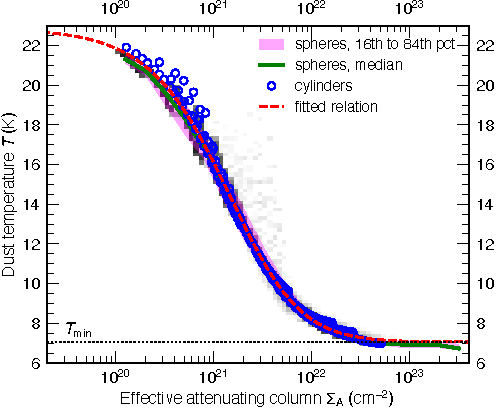
\includegraphics[width=0.95\columnwidth]{fig_shielding.pdf}
\caption{The dust temperature against the effective attenuating column $\Sigma_{\rm A}$ in the radiative transfer models. The gray
scale shows the distribution of the radial shells (over $10^5$) of the $2086$ spheres in this plane, each shell weighted by its
mass, with every sphere given the same total weight. The gray scale is logarithmic and spans four orders of magnitude. The green
solid line and the magenta band are, respectively, the weighted median and the 16th to 84th percentiles of the temperature in bins
of $0.2$\,dex in $\Sigma_{\rm A}$. The blue circles correspond to the $45$ radii of each of the seven cylinders. The red dashed
line is the relation of Eq.~(\ref{eq:law}), fitted to the spheres and the cylinders with equal total weights. The dotted line marks
the temperature $T_{\rm min}$ that fully shielded dust approaches.}
\label{fig:shielding}
\end{figure}

\subsection{Dependence of dust temperature $T$ on $\Sigma_{\rm A}$}
\label{sec:relation}

%%%%% -----------------------------------------------------------------------------------------------------------------------------
%%%%% NUMBERS (2026-10-20): 2.4 K is the mass-weighted mean excess over the relation of the outermost shells of the spheres in the
%%%%% densest embedding clouds (cSD_09), measured on attenuation_law.txt of the fit with the outermost shells kept (-keepouter);
%%%%% the shells were identified with the node column of the table and diagnose_shielding_branches.py.
%%%%% -----------------------------------------------------------------------------------------------------------------------------
The relation between $\Sigma_{\rm A}$ and $T$ is not a free choice. It follows from radiative transfer, once the dust properties
and the external radiation field are fixed. The density and the dust temperature of every model are tabulated in radial shells, the
cells of its radial grid: spherical shells for the cores and cylindrical shells at $45$ radii for the filaments. The attenuating
column of a shell was computed by integrating the number density of hydrogen molecules along many rays, $240$ directions for the
cores and $200{\times}180$ directions of equal solid angle for the filaments, and Eq.~(\ref{eq:seff}) was then evaluated by summing
over the directions. A few innermost shells of the densest cores, with poor Monte Carlo statistics, and the outermost shell of
every sphere, whose single temperature is an average over a steep gradient, were rejected (Appendix~\ref{sec:grid}).
%%The density structure of every model is known, and the attenuating column of a shell
%%was computed by integrating the number density of hydrogen molecules along many rays: $240$ directions for the spherical shells of
%%the cores and $200{\times}180$ directions of equal solid angle for the cylindrical shells of the filaments, at $45$ radii.
%%Equation~(\ref{eq:seff}) was then evaluated by summing over the directions. 

%%%%% -----------------------------------------------------------------------------------------------------------------------------
%%%%% NUMBERS (2026-10-20): T_min, T_max, Sigma_star, gamma and the scatter from the header of attenuation_law.txt written by
%%%%% fit_attenuation_law.py (2086 spheres without their outermost shells, 7 isolated cylinders, equal weights). The departures
%%%%% of the spheres and cylinders and the leave-one-cylinder change of the factor from python/paper_numbers/law_checks.py with
%%%%% attenuation_law.txt and attenuation_law-leave_one_cylinder_out.txt (the seven fits run with fit_attenuation_law.py,
%%%%% one cylinder left out each).
%%%%% -----------------------------------------------------------------------------------------------------------------------------
More than $10^5$ shells of the $2086$ spheres and $45$ shells of each of the seven cylinders follow a single relation
(Fig.~\ref{fig:shielding}) that can be fitted with the function
\begin{equation}
  T(\Sigma_{\rm A}) = T_{\rm min} + \left(T_{\rm max} - T_{\rm min}\right) \left(1 + \Sigma_{\rm A}/{\Sigma_\star}\right)^{-\gamma},
\label{eq:law}
\end{equation}
where the fit parameters are $T_{\rm min\!} = 7.0495$\,K, $T_{\rm max\!} = 22.8668$\,K, $\Sigma_{\star\!} =
2.3897{\times}10^{21}$\,cm$^{-2}$ and $\gamma = 1.5969$. The fit minimized the mass-weighted sum of the squared logarithmic
differences between the fitted and the model temperatures, with every sphere and every cylinder normalized to the same total weight
and the two types of structure given equal weights. The mass-weighted scatter about the relation is $2.4$\%. The cores and the
filaments follow the same relation: on average, the cores are $0.6$\% colder than the relation and the filaments $0.1$ to $1.1$\%
warmer. Leaving out any single filament changes the correction factor by at most $1.5$\%. Above $\Sigma_{\rm A\!}\approx
10^{23}$\,cm$^{-2}$, the models contain too little mass to constrain the relation.

\begin{figure*}
\centering
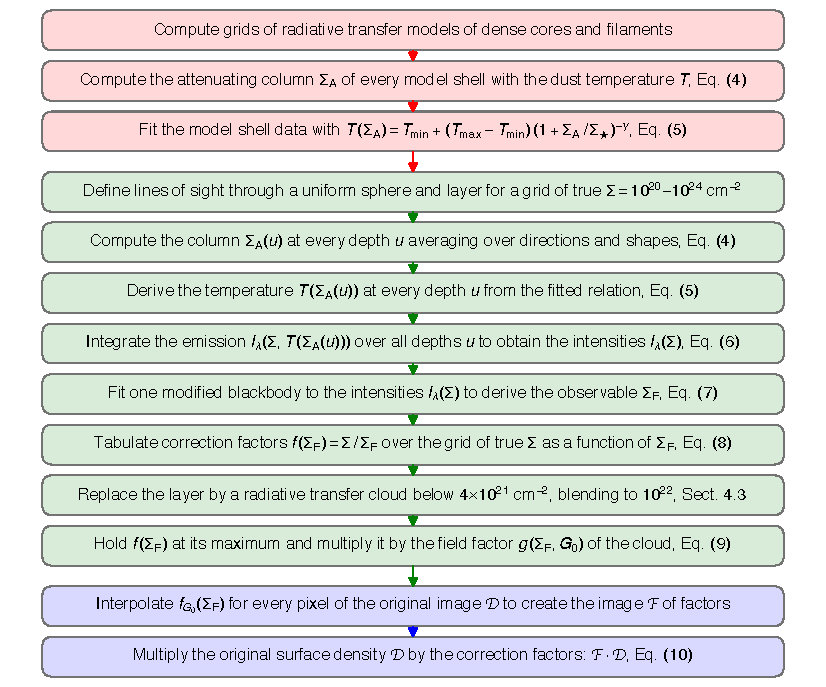
\includegraphics[width=0.76\textwidth]{fig_method.pdf}
\caption{Flowchart of the method. The first group is the calibration, which is done once and yields the temperature relation of
Eq.~(\ref{eq:law}). The second is the calculation of Sect.~\ref{sec:factor}, repeated for a grid of true surface densities
$\Sigma$, which yields the table of the correction factor against the surface density that an observed image actually holds. Its
last two steps calibrate the low surface densities on a radiative transfer model of a diffuse cloud (Sect.~\ref{sec:diffuse}) and
adapt the factor to the radiation field of the cloud (Sect.~\ref{sec:g0corr}). The third group is what is then done to an image, at
any resolution.}
\label{fig:method}
\end{figure*}

The two limits have simple meanings. $T_{\rm max}$ is the temperature of dust that the radiation reaches without attenuation.
$T_{\rm min}$ is the temperature that dust approaches when the ultraviolet and optical radiation no longer reach it. The dust is
then heated only by the infrared radiation that still penetrates, including the emission of the warmer dust around it, and by the
cosmic microwave background. Between the two limits, $\Sigma_\star$ is the characteristic attenuating column of the decline: at
$\Sigma_{\rm A\!} = \Sigma_\star$, the excess of the temperature over $T_{\rm min}$ is reduced by the factor $2^{\gamma\!}\approx
3$, and $\gamma$ sets how steeply the temperature falls at larger columns.

A single relation describes models that differ greatly from one another. This is the result that makes the surface density
correction method possible. The size of a core and its concentration do not appear in Eq.~(\ref{eq:law}), and they do not need to.
They affect the temperature only by changing the amount of material between the dust and the radiation. For the same reason, the
filaments did not need a surrounding cloud. A cloud changes the temperatures near the edge of a structure, but $\Sigma_{\rm A}$ of
every dust grain already includes all the material that shields it, whatever its origin. Accordingly, the cores, embedded in clouds
that differ by a factor of $256$ in surface density, follow the same relation. The cylinders add the shielding geometry of a
filament. An isolated cylinder provides this geometry without an artificial envelope, whereas a cylindrical envelope shields the
axis less than a cloud layer of the same surface density (Appendix~\ref{app:embfil}). 

The scatter of $2.4$\% about the relation measures how much structures of different shapes and in different embedding clouds differ
at the same $\Sigma_{\rm A}$. It reflects the physics that a single gray $\Sigma_{\rm A}$ omits, mainly the wavelength dependence
of the extinction, and the scatter would not decrease with more models.

% =====================================================================

\section{The correction method}
\label{sec:corr}

\subsection{The correction factor for uniform structures}
\label{sec:factor}

The correction factor $f$ is the ratio of the true surface density $\Sigma$ of a line of sight to the surface density $\Sigma_{\rm
F}$ obtained by fitting a single-temperature modified blackbody to the intensities $I_{\lambda}$ emerging along that line of sight.
It was computed for a grid of values of the true surface density $\Sigma$, from $10^{20}$ to $10^{24}$\,cm$^{-2}$ in logarithmic
steps. Apart from the calibration of diffuse material (Sect.~\ref{sec:diffuse}), the derivation has no free parameters.

Calculating $f$ requires a model of the distribution of the material along the line of sight. Two bodies of uniform density with
the same surface density $\Sigma$ were adopted: a sphere, seen through its center, and a plane-parallel layer, seen along its
normal. Each line of sight was divided into short segments. The position of a segment is given by $u$, which is the fraction of
$\Sigma$ that lies in front of it, from $u = 0$ at the near surface to $u = 1$ at the far surface. The factor was computed in five
steps (Fig.~\ref{fig:method}).

(1) The effective attenuating column $\Sigma_{\rm A}$ of every segment was computed from Eq.~(\ref{eq:seff}), separately for the
sphere and the layer. The two values were averaged for each segment, for the reason given in Sect.~\ref{sec:orient}, giving a
single profile $\Sigma_{\rm A}(u)$ for the line of sight.

(2) The dust temperature of every segment followed from $\Sigma_{\rm A}(u)$ and the relation of Eq.~(\ref{eq:law}). The
temperature is therefore highest at the two surfaces of the line of sight and lowest in its middle, where $\Sigma_{\rm A}$ is
largest.

(3) The intensity $I_{\lambda}$ emerging from the line of sight was obtained by integrating the emission of all its segments,
\begin{equation}
   I_\lambda(\Sigma) = \kappa_\lambda\,\eta\,\muH\,\mH\,\Sigma \int_0^1 B_\lambda \big(T(\Sigma_{\rm A}(u))\big)\,{\rm d}u,
\label{eq:emission}
\end{equation}
where $\kappa_\lambda$ is the dust opacity per unit mass of dust, $\eta = 0.01$ is the dust-to-gas mass ratio, $\muH = 2.8$ is the
mean molecular weight per hydrogen molecule, and $\mH$ is the mass of a hydrogen atom.

(4) A single modified blackbody was fitted to these intensities exactly as \emph{hires} fits the observed images: in the same
wavebands, from $160$ to $500${\um}, and with the same weights, inversely proportional to the squares of the calibration
uncertainties, $20$\% at $160${\um} and $10$\% at $250$ to $500${\um} \citep{Konyves+2015}. The fit gave a temperature $T_{\rm F}$,
and the surface density $\Sigma_{\rm F}$ for this line of sight was derived from the intensity $I_{\rm ref}$ at the reference
wavelength $\lambda_{\rm ref\!}=500${\um}, at which $\Sigma_{\rm F}$ is least sensitive to the temperature (cf.
Eq.~(\ref{eq:sensitivity})):
\begin{equation}
   \Sigma_{\rm F}(\Sigma) = \frac{I_{\rm ref}(\Sigma)} {\kappa_{\rm ref}\,\eta\,\muH\,\mH\,B_{\rm ref}(\Teff)}.
\label{eq:fitted}
\end{equation}

(5) The correction factor is the ratio of the true and fitted surface densities. An observed image contains $\Sigma_{\rm F}$, not
$\Sigma$, so the factor was tabulated against $\Sigma_{\rm F}$:
\begin{equation}
   f(\Sigma_{\rm F}) = {\Sigma}/{\Sigma_{\rm F}}.
\label{eq:factor}
\end{equation}

\begin{figure}
\centering
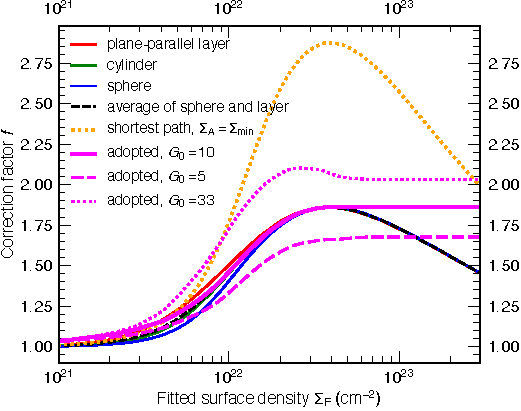
\includegraphics[width=0.98\columnwidth]{fig_relation.pdf}
\caption{The correction factor as a function of the surface density $\Sigma_{\rm F}$ of the uncorrected image for three uniform
structures -- plane-parallel layer, cylinder, and uniform sphere -- and for an average of the sphere and layer, with $G_0 = 10$.
The dotted curve uses the column $\Sigma_{\rm A}=\Sigma_{\rm min}$ along the shortest path instead of the angular average
(Appendix~\ref{app:shape}). The thick magenta curve is the adopted relation for $G_0 = 10$. Below $3.98{\times}10^{21}$\,cm$^{-2}$
it replaces the analytic layer by a radiative transfer model of a diffuse cloud (Sect.~\ref{sec:diffuse}), and above its maximum it
is held constant (Sect.~\ref{sec:factor}). The thin magenta curves are the adopted relation for $G_0 = 5$ and $33$, with the field
factor of Eq.~(\ref{eq:factorg0}).}
\label{fig:relation}
\end{figure}

Figure~\ref{fig:relation} shows the result. For the analytic structures, the factor is unity below $10^{21}$\,cm$^{-2}$, where
nothing is attenuated. It rises steeply through the range of surface densities of most of a molecular cloud. It reaches its
maximum, $1.86$, near $4{\times}10^{22}$\,cm$^{-2}$ and then declines, to $1.45$ at $3{\times}10^{23}$\,cm$^{-2}$. The factor is
largest when a line of sight contains both a warm surface layer, which dominates the emission, and a cold interior that holds most
of the mass. The surface layer has a nearly fixed surface density of a few $10^{21}$\,cm$^{-2}$, set by the depth to which the
heating radiation penetrates. Up to about $4{\times}10^{22}$\,cm$^{-2}$, the cold interior grows with $\Sigma$, and so does the
bias of the fit. At higher surface densities, most of the material of a uniform body has reached the temperature floor $T_{\rm
min}$. The cold interior then dominates the emission as well as the mass, the fitted temperature approaches $T_{\rm min}$, and the
line of sight becomes nearly isothermal again, so the factor declines toward unity.

Real dense structures are not uniform. A concentrated core has a cold center inside a warmer envelope, and its temperature still
varies along the line of sight. The radiative transfer models confirm this: the factor that they require stays between $2.0$ and
$2.4$ up to the highest surface densities of the models, ${\sim}10^{23}$\,cm$^{-2}$. The decline of the analytic relation is an
artifact of the uniform bodies. The factor was therefore held at its maximum above the surface density at which it is reached, so
that it never decreases with the surface density. The adopted relation differs from the analytic one in this respect and below
$10^{22}$\,cm$^{-2}$, for the reason given in Sect.~\ref{sec:diffuse}.

\subsection{Weak dependence on shapes and density distributions}
\label{sec:orient}

The correction factor assumes specific shapes of structures, however those in an observed region are unknown. Cores are embedded in
filaments, filaments are curved and blended with their neighbors, and everything lies in a fluctuating background. Fortunately, the
surface density correction depends little on the adopted shape.

Figure~\ref{fig:relation} shows the correction factor for a uniform sphere, cylinder, and plane-parallel layer of the same observed
surface density. The three agree to within $10$\% everywhere. Outside the range from $2.5{\times}10^{21}$ to
$1.3{\times}10^{22}$\,cm$^{-2}$, they agree to within $5$\%. This is because at low surface densities the attenuation is weak, the
line of sight is nearly isothermal, and every shape gives $f \approx 1$. At high surface densities the deepest material is
optically thick in every direction, and the distribution of path lengths no longer matters (Fig.~\ref{fig:geometry}). Shapes of
structures matter only in between, where the correction itself is modest. This is why the sphere and the layer were averaged in
Sect.~\ref{sec:factor}, and half of their difference, at most $5$\%, was regarded as the uncertainty due to the geometry. A uniform
cylinder seen perpendicular to its axis lies between the two limits, and its factor is within $1.5$\% of their average, so the
average also represents filaments. The factor was computed for central lines of sight, along the normal of a layer and the diameter
of a sphere. Off-center lines of sight through a sphere or a filament pass closer to its surface. They are warmer and more
nearly isothermal than a central line of sight with the same $\Sigma$, and they are slightly over-corrected. The validation on all
pixels of the models includes this effect (Sect.~\ref{sec:valgrid}). Inclined layers and filaments are over-corrected too
(Appendix~\ref{sec:incl}). Appendix~\ref{app:shape} explains why the sphere and the layer are the two limits and why $\Sigma_{\rm
A}$ cannot be replaced by $\Sigma_{\rm min}$.

One assumption remains: each structure was assumed to have a uniform density. This assumption matters much less than it seems. For
a line of sight through a plane-parallel layer, in which the density varies only along the line of sight, it does not matter at
all. A dust grain is shielded by the column between the grain and the surface. This column does not depend on how the material
within it is distributed. Measured in column rather than in depth, every segment of a line of sight contains the same mass,
whatever the density profile; the density only sets how long the segment is. Equation~(\ref{eq:emission}), written in the fraction
$u$ of the column in front of a segment, therefore holds for any density profile, and the density does not appear there. Two lines
of sight with the same total surface density emit the same spectrum, whether their material is smooth or clumped and wherever a
clump lies. Appendix~\ref{app:arrange} confirms this numerically, showing that density profiles that differ by a factor of thirty
reproduce the smooth case to within $0.02$\%.

This argument holds for a layer, in which radiation reaches the dust only through the material along the line of sight. In a
bounded structure, radiation also reaches the dust from the sides, and only through this effect do the concentration and
arrangement of the material matter. Their effect is modest. A sphere with a central-to-edge density ratio of $10$ needs a
correction $2$ to $5$\% larger than a uniform sphere of the same central surface density. For a ratio of $10^3$, it needs $9$ to
$20$\% more, and the difference grows with the surface density. A structure embedded at an unknown depth in a diffuse cloud is a
different case. In the extreme cases, the correction for such a line of sight is $13$\% too small, for a structure in a weak cloud,
or $21$\% too large, for a structure at a face of a dense cloud. These cases are not typical: near the middle of a cloud, the error
is only a few percent, and in the simulated sky it is about $10$\% (Sect.~\ref{sec:sim}). Both effects are measured in
Appendix~\ref{app:arrange}, and they enter the uncertainties of Appendix~\ref{sec:limits}.

\subsection{Calibration on a diffuse cloud at low surface densities}
\label{sec:diffuse}

The relation of Eq.~(\ref{eq:law}) was determined for bounded structures (spheres and cylinders). Most of the area of molecular
clouds is covered by diffuse material, so the correction factor $f$ was also calibrated on the radiative transfer model of the
diffuse cloud (Sect.~\ref{sec:modcloud}). For each line of sight (pixel) of this model, one modified blackbody was fitted to the
intensities at $160$ to $500${\um}, and the result was compared with the true surface density.

The analytic layer, which enters the average of Sect.~\ref{sec:orient}, does not reproduce the correction factors that the
radiative transfer model of the cloud requires. The layer needs almost no correction below $10^{21}$\,cm$^{-2}$, but the cloud
needs $5$\% even at $3.5{\times}10^{20}$\,cm$^{-2}$ and $15$--$25$\% at $2$--$4.5{\times}10^{21}$\,cm$^{-2}$. The reason is the
surface of the cloud, whose outer layers are heated by the unattenuated ultraviolet radiation from half the sky. They are up to
$3$\,K warmer than Eq.~(\ref{eq:law}) predicts, because that relation describes the attenuation with a single gray opacity. The
temperature therefore varies more along a line of sight through the cloud than through the analytic layer.

The analytic layer was therefore replaced by the radiative transfer model of the cloud at low surface densities. Below a fitted
surface density of $3.98{\times}10^{21}$\,cm$^{-2}$, the factor was set to the average of the analytic sphere and of the factor
measured on the cloud. Between $3.98{\times}10^{21}$ and $10^{22}$\,cm$^{-2}$, it was blended smoothly into the analytic average of
sphere and layer, which was used above. Extending the calibration on the cloud to higher surface densities was tested and rejected:
it improved the cloud by only $2$\%, did not improve the flanks of the dense filaments in the simulated sky, and over-corrected
dense cores. The factor remains a function of the surface density alone. The bounded spheres and the extended cloud are the two
limits for diffuse material, as the sphere and the layer are for a single structure. Their average divides the uncertainty between
them. As a result, the uniform clouds around the cores are corrected about $2$\% too much and the model of the diffuse cloud $11$\%
too little in the median (Sects.~\ref{sec:valgrid} and \ref{sec:sim}).

\subsection{Adaptation to different radiation fields}
\label{sec:g0corr}

The relation of Eq.~(\ref{eq:law}) and the correction factor $f$ were calibrated for $G_0 = 10$. However, different clouds are
heated by radiation of very different strengths. The diffuse material of the molecular clouds listed in Appendix~\ref{app:fieldest}
requires fields from $G_0 \lesssim 1$ to ${\sim}250$. A stronger field heats the dust at every attenuating column, and it changes
the temperature contrast along the line of sight, of which $T_{\rm max}/T_{\rm min}$ is the largest value.
The factor that a line of sight requires therefore depends on the
field (Appendix~\ref{sec:field}).

This dependence was measured on the model grid of embedded cores (Sect.~\ref{sec:modcores}) for nine radiation fields from $G_0 =
0.98$ to $483$. For each field, the factors that the pixels of all its models required were averaged over the pixels with similar
fitted surface densities, which gives the mean factor as a function of $\Sigma_{\rm F}$. The ratio of this mean to the same mean at
$G_0 = 10$ is the field factor $g(\Sigma_{\rm F}, G_0)$ (Fig.~\ref{fig:fieldfactor} and Appendix~\ref{app:fieldR}). Above
$7.1{\times}10^{22}$\,cm$^{-2}$, the grid contains too few pixels to determine it, and $g$ was held at its value there. Between the
radiation fields, $\log g$ is interpolated linearly in $\log G_0$. The field factor is close to unity in diffuse material and
departs from it most above ${\sim}10^{22}$\,cm$^{-2}$. It is largest for $G_0 \approx 50$, and in the strongest fields it falls
below unity at high surface densities (Appendix~\ref{app:field}).

The non-monotonic dependence on the field strength follows from how the relation of Eq.~(\ref{eq:law}) changes with it
(Appendix~\ref{app:fieldR}). In fields up to $G_0 \approx 50$, a stronger field warms the unattenuated dust much more than the
shielded dust, and the larger temperature contrast along a line of sight increases the bias. In stronger fields, the shielded dust
is warmed too, which reduces the contrast, and warmer dust makes the Planck function at the wavelengths of the fit less sensitive
to the temperature, which reduces the bias of any contrast.

\begin{figure}
\centering
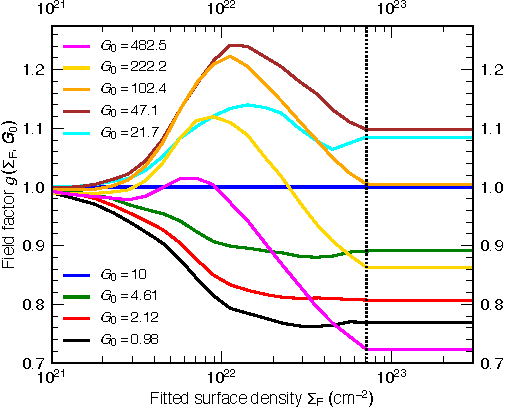
\includegraphics[width=0.98\columnwidth]{fig_fieldfactor.pdf}
\caption{The radiation field factor $g(\Sigma_{\rm F}, G_0)$ from Eq.~(\ref{eq:factorg0}) is plotted against the fitted surface
density $\Sigma_{\rm F}$, for the nine field strengths $G_0$ of the model grid, from the weakest to the strongest. For the field 
$G_0 = 10$ of the calibration, $g = 1$. Above $7.1{\times}10^{22}$\,cm$^{-2}$ (dotted line), $g$ is held constant.}
\label{fig:fieldfactor}
\end{figure}

The surface density correction factor for a cloud in the radiation field with $G_0$ is
\begin{equation}
  f_{G_0}(\Sigma_{\rm F}) = g(\Sigma_{\rm F}, G_0) \,\max_{\Sigma^{\prime} \le \Sigma_{\rm F}} f(\Sigma^{\prime}),
\label{eq:factorg0}
\end{equation}
where the maximum holds the factor for uniform bodies at its maximum (Sect.~\ref{sec:factor}). The field factor is not held at its
maximum (Fig.~\ref{fig:fieldfactor}), because its decline in strong fields is measured on the radiative transfer models. The field
strength $G_0$ is a single number for a cloud. It is the value that the models require to reproduce the observed temperatures, an
effective field for the model dust, which can differ from the physical field. It is estimated from the temperatures of the diffuse
material of the whole map, with the procedure of Appendix~\ref{app:fieldest}. It is not read from the temperature of each pixel,
which is ambiguous (Appendix~\ref{app:tcorr}). The correction therefore still depends on the surface density alone, and the field
is an input of the method, like the wavebands.

\subsection{Correcting surface density images}
\label{sec:apply}

An observed surface density image is corrected by multiplying it by the image of the correction factors computed from the image
itself,
\begin{equation}
  \Dimc = \mathcal{F}\,\Dim, \quad \mathcal{F} \equiv f_{G_0\!}\left(\Dim\right),
\label{eq:correction}
\end{equation}
where $f_{G_0\!}$ of Eq.~(\ref{eq:factorg0}) is evaluated pixel by pixel. By design, the correction factor is a function of only
two quantities, the surface density of a pixel and the radiation field strength $G_0$. It was calibrated for the surface density
that a single modified blackbody fit returns at the resolution of the longest waveband, $O = 36.3{\arcsec}$. When no estimate of
$G_0$ is supplied, the default $G_0 = 10$ is used.

The correction method also applies to higher-resolution surface density images (with $O<36.3${\arcsec}). Evaluated on the much
sharper \emph{hires} images at $O = 13.5{\arcsec}$, the correction factor $f_{G_0\!}(\Dim)$ gives core masses $5$\% higher, and
closer to the truth, than when it is evaluated at $O = 36.3{\arcsec}$, and a smaller underestimation at the core centers
(Table~\ref{tab:valgrid}). On the cloud of the simulated sky, the two agree to $0.5$\%. The factor is therefore evaluated on the
image that is corrected. What \emph{hires} adds, and no correction can replace, is the information on scales finer than the beam of
the longest waveband. Only the final images produced by \emph{hires} can be corrected, not the intermediate ones, because the
latter are fitted to fewer wavebands. The correction method is a \emph{Fortran} utility \emph{hicorrect} belonging to the source
and filament extraction method \emph{getsf} and is available on its
webpage\footnote{\url{http://irfu.cea.fr/Pisp/alexander.menshchikov/}}.

\subsection{Requirements of the correction method}
\label{sec:needs}

The order of operations matters when an image is separated into its structural components, such as sources, filaments, and their
backgrounds \citep[e.g., with \emph{getsf},][]{Menshchikov2021method}. A dust grain is shielded by the whole column along its line
of sight, so the correction factor must be evaluated on the total surface density, not on a component of it. The image must
therefore be corrected first, and the components separated afterwards. If a background is subtracted first, the factor is evaluated
at a surface density that the material does not have, and the structure is corrected much too little. For the same reason, the
correction must never be applied to an image that is already corrected, or to a true surface density.

One condition applies when the correction is used outside \emph{hires}. The correction factor $f$ of Eq.~(\ref{eq:factor}) is built
for the wavebands and the weights of the fit (Sect.~\ref{sec:factor}), because $\Sigma_{\rm F}$ depends on both. For uniform
bodies, a map fitted with equal weights is under-corrected by $6$--$15$\% above $10^{22}$\,cm$^{-2}$, one fitted without $160${\um}
is over-corrected by $12$--$24$\%, and one whose fit includes $70$ or $100${\um} is under-corrected by up to $40$\%. The relation
cannot be replaced by anything derived from the photometry itself, because the mixing of temperatures along a line of sight changes
the spectral shape by only a few percent (Appendix~\ref{app:colors}).

Surface density images are sometimes derived from other sets of wavebands or with other weights, for example from the
$250$--$500${\um} wavebands alone or with $70$ and $100${\um} included. To correct such images, the code computes the correction
factor of the uniform sphere and layer (Sect.~\ref{sec:factor}) for the wavebands and weights given, and at low surface densities
it combines that factor with a calibration on the cloud model (Sect.~\ref{sec:diffuse}) computed for the same set:
$160$--$500${\um} with the standard or equal weights, $250$--$500${\um}, $100$--$500${\um} and $70$--$500${\um}. The field factor
was measured with the standard set only. For $160$--$500$ and $250$--$500${\um} it is accurate to within $5$\% in fields $G_0
\lesssim 50$ and to within $16$\% in the strongest fields. For sets that include $70$ or $100${\um}, the error reaches $17$\%. The
effects of noise and of calibration errors are discussed in Appendix~\ref{sec:calerr}.

% =====================================================================

\section{Validation of the method}
\label{sec:valid}

The method can be tested only on images whose true surface density is known. The correction was tested in three settings, all
computed with radiative transfer. The first is a grid of models of cores, each embedded in its own uniform cloud. The second is a
set of isolated filaments. The third is a simulated sky, in which a cloud, filaments and cores overlap along the lines of sight.
All of them were computed for $G_0 = 10$, hence $g = 1$ in Eq.~(\ref{eq:factorg0}). Holding the factor $f$ at its maximum changes
it only above $4.0{\times}10^{22}$\,cm$^{-2}$. Within the surface densities of these models, the change is at most $2$\%, and the
results below are given without it. The correction for other fields was tested separately (Appendix~\ref{sec:field}).

\subsection{Models of embedded cores}
\label{sec:valgrid}

The correction was validated on the $1815$ spherical models from the subdivision grid (Sect.~\ref{sec:modcores}), which were not
used to fit the relation of Eq.~(\ref{eq:law}). The image $\Dim_{13.5}$ of each embedded core was corrected with
the factors $\mathcal{F}_{13.5}$ evaluated on that image and, for comparison, with the factors $\mathcal{F}_{36.3}$ evaluated on
$\Dim_{36.3}$. The corrected images were compared with the true surface density at the same resolution.

Table~\ref{tab:valgrid} presents four quantities. The total surface density was integrated over the true model footprint, defined
as the area within the contour at $1$\% of the peak of the core in its true image at $O = 13.5{\arcsec}$. The core mass $M$ was
integrated after subtraction of the background, defined as the median surface density in a ring $15{\arcsec}$ wide just outside the
footprint. The mass could be measured for $1750$ of the models (Appendix~\ref{sec:grid}). Both are given as accuracy ratios, the
corrected value divided by the true one. The relative error of the corrected surface density is given at $3$ and $21{\arcsec}$
from the center of the core, and its radial profile is shown in Fig.~\ref{fig:valgrid}.

\begin{table}
%%%%% -----------------------------------------------------------------------------------------------------------------------------
%%%%% NUMBERS (2026-10-20): Table tab:valgrid and the numbers of Sect. 5.1 are from validate3_finRTlaw.txt, written by
%%%%% validate_calib3.py on the subdivision grid: rows 'hicorrect2, fine' (factor at 13.5 arcsec) and 'hicorrect2, coarse' (36.3);
%%%%% Center and 21 arcsec from the radial table at 3 and 21 arcsec; the footprint errors from the table of the misjudged footprint.
%%%%% -----------------------------------------------------------------------------------------------------------------------------
\caption{Validation of the corrections on $1815$ radiative transfer models of embedded cores that were not used to fit the relation
of Eq.~(\ref{eq:law}).}
\label{tab:valgrid}
\centering
\begin{tabular}{@{}l@{\hspace{6pt}}c@{\hspace{6pt}}c@{\hspace{6pt}}c@{\hspace{6pt}}c@{}}
\hline\hline
\noalign{\smallskip}
\,Image\tablefootmark{a} & Total\tablefootmark{b} & Core mass\tablefootmark{c} &\!\! Center\tablefootmark{d} 
&\!\!\! $21{\arcsec}$\tablefootmark{e}\\
\noalign{\smallskip}
\hline
\noalign{\smallskip}
\,$\Dim_{13.5}$                     & 0.78 (0.56--0.93) & 0.63 (0.46--0.86) &\!\!\! $-0.44$ &\!\!\! $-0.21$\,\\
\,$\mathcal{F}_{13.5\,}\Dim_{13.5}$ & 0.99 (0.92--1.03) & 0.98 (0.75--1.11) &\!\!\! $-0.13$ &\!\!\! $+0.02$\,\\
\,$\mathcal{F}_{36.3\,}\Dim_{13.5}$ & 0.98 (0.90--1.02) & 0.93 (0.70--1.08) &\!\!\! $-0.16$ &\!\!\! $+0.01$\,\\
\noalign{\smallskip}
\hline
\end{tabular}
\tablefoot{
\tablefoottext{a}{The images before the correction and after it, with the factors evaluated at $O = 13.5$ or $36.3{\arcsec}$.}
\tablefoottext{b}{The accuracy ratio of the total surface density over the true model footprint: the median over the models, with
the 16th and 84th percentiles in parentheses.}
\tablefoottext{c}{The accuracy ratio of the core mass, for the $1750$ models in which it can be measured: the median and
percentiles as in (b).}
\tablefoottext{d}{The median relative error of the surface density at $3{\arcsec}$ from the center of the core.}
\tablefoottext{e}{The same at $21{\arcsec}$ from the center.}
}
\end{table}

\begin{figure*}
\centering
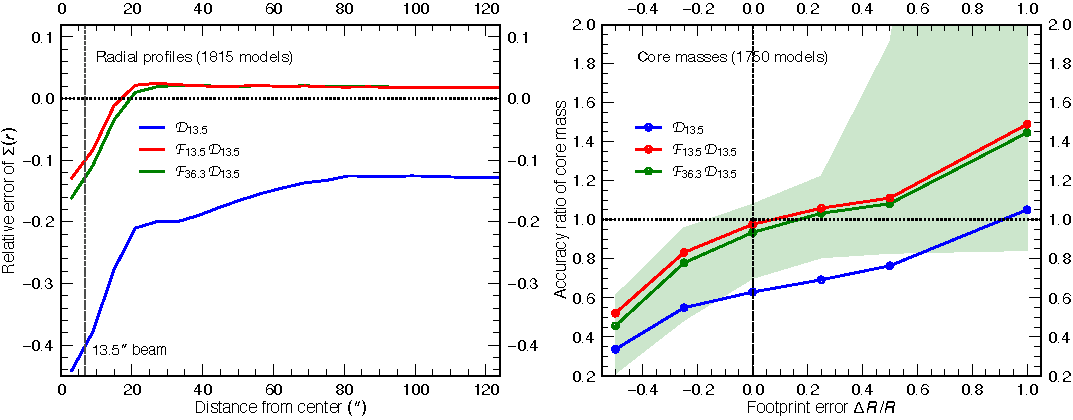
\includegraphics[width=0.96\textwidth]{fig_grid_validation.pdf}
\caption{The correction tested on $1815$ radiative transfer models that were not used to fit the relation of Eq.~(\ref{eq:law}).
\emph{Left}: The relative error of the corrected surface density (Sect.~\ref{sec:valgrid}), against the distance from the center of
the core, as the median over the models. The dashed line marks $O/2$ for $O = 13.5{\arcsec}$. \emph{Right}: The accuracy ratio
of the core mass, for the $1750$ models in which it can be measured, when the estimated radius $R$ of the core, and hence of its
footprint, is too small ($\Delta R < 0$) or too large ($\Delta R > 0$). The background is always taken in a ring just outside the
footprint used. The lines are medians over the models, and the band marks the 16th to 84th percentiles for
$\mathcal{F}_{36.3\,}\mathcal{D}_{13.5}$.}
\label{fig:valgrid}
\end{figure*}

The uncorrected image $\Dim_{13.5}$ contains $78$\% of the true surface density and $63$\% of the core mass. The largest
underestimation, $44$\%, is at the core center. The correction restores the median total to $99$\% and the median core mass to
$98$\%. Beyond $15{\arcsec}$ from the center, the corrected surface density is about $2$\% too high (Fig.~\ref{fig:valgrid}).
There, the surface density is dominated by the uniform cloud around the core, which the calibration of Sect.~\ref{sec:diffuse}
corrects slightly too much. An underestimation of $13$\% remains at $3{\arcsec}$ from the centers of the cores. No correction that
depends on the surface density alone can remove it. The center of a core is colder than the center of a uniform structure with the
same surface density, and the surface density does not reveal this. The factor evaluated at $36.3{\arcsec}$ gives almost the same
integrated values but a larger underestimation at the center (Sect.~\ref{sec:apply}).

The errors of individual models are larger than the median errors. For $16$\% of the cores, the corrected mass is more than $25$\%
too low, and for another $16$\%, it is more than $11$\% too high (Table~\ref{tab:valgrid}). The errors depend on the contrast of a
core, the ratio of its peak to the background. Cores with contrasts above $10$ dominate their lines of sight, and their cold
interiors leave the surface density at their centers underestimated by $45$\% and their masses by $16$\%. Cores with contrasts
below $1.5$ are nearly uniform and are corrected to within $4$\%. No correction that depends on the surface density alone can
remove this spread, because cores with the same surface density differ in how their temperature varies along the line of sight.

In observed images, the footprints of cores are estimated by source extraction and can be wrong. To test the effect of such errors,
the radius $R$ of the footprint was decreased or increased by $\Delta R$ (Fig.~\ref{fig:valgrid}). A footprint too small by $\Delta
R/R$ of $0.25$ or $0.5$ lowers the median corrected mass from $0.98$ to $0.83$ or $0.52$, because part of the core is then
considered as background. A footprint too large by $0.25$ or $0.5$ raises it to $1.06$ or $1.11$, and the spread widens sharply for
cores of low contrast, whose mass is small compared with the background within the footprint. For contrasts below $1.5$, a
footprint too large by $\Delta R/R = 1$ triples the median mass, whereas for contrasts above $10$ it lowers it by $12$\%. These
errors are lower limits, because the models are embedded in uniform clouds, whereas real cores overlap with filaments, background
fluctuations, and other cores, which make the background harder to estimate.

\subsection{Models of filaments}
\label{sec:cyl}

The correction was also validated on the seven cylindrical filaments of Sect.~\ref{sec:modfil}. Their surface density images
$\Dim_{13.5}$, derived with \emph{hires} from the simulated emission, were corrected with the factors $\mathcal{F}_{13.5}$
evaluated on them and compared with the true surface density at the same resolution. They are isolated, so their profiles are not
confused by any background. Table~\ref{tab:cyl} and Fig.~\ref{fig:cylinders} give the results, measured on the median profile
over the middle part of each cylinder.

\begin{table*}
%%%%% -----------------------------------------------------------------------------------------------------------------------------
%%%%% NUMBERS (2026-10-20): Table tab:cyl and the numbers of Sect. 5.2 from python/paper_numbers/cylinder_table.py on the seven
%%%%% *_isolated directories (mc.surfdens.fits and hi.surface.density.r13p5.fits; the factor is applied to the median profile,
%%%%% as in fig_cylinders).
%%%%% -----------------------------------------------------------------------------------------------------------------------------
\caption{The isolated radiative transfer cylinders at $O = 13.5{\arcsec}$. $\Sigma_0$: the true surface density on the axis. Crest: the
accuracy ratio of the surface density on the axis, before and after the correction. $\Lambda$: the accuracy ratio of the linear
density within $\pm300{\arcsec}$, before and after. $H$: the half-maximum width of the true, the uncorrected and the corrected
profile. $\alpha$: the slope of $\log\Sigma$ against $\log r$ between $20$ and $120{\arcsec}$ from the crest, for the same three
profiles.}
\label{tab:cyl}
\centering
\begin{tabular}{lcccc}
\hline\hline
\noalign{\smallskip}
$\Sigma_0$ (cm$^{-2}$) & Crest & $\Lambda$ & $H$ (${\arcsec}$) & $\alpha$ \\
\noalign{\smallskip}
\hline
\noalign{\smallskip}
$3{\times}10^{21}$                  & 0.86 $\rightarrow$ 0.94 & 0.96 $\rightarrow$ 1.01 & \!48\, \,\,\,58\,\, 55  & 0.89\,\, 0.88\,\, 0.90 \\
$1{\times}10^{22}$                  & 0.66 $\rightarrow$ 0.83 & 0.87 $\rightarrow$ 0.97 & \!48\, \,\,\,71\,\, 61  & 0.89\,\, 0.81\,\, 0.87 \\
$3{\times}10^{22}$                  & 0.50 $\rightarrow$ 0.80 & 0.75 $\rightarrow$ 0.94 & \!48\, \,\,\,79\,\, 60  & 0.89\,\, 0.70\,\, 0.85 \\
$5{\times}10^{22}$                  & 0.46 $\rightarrow$ 0.81 & 0.68 $\rightarrow$ 0.94 & \!48\, \,\,\,75\,\, 60  & 0.89\,\, 0.67\,\, 0.87 \\
$1{\times}10^{23}$                  & 0.42 $\rightarrow$ 0.78 & 0.60 $\rightarrow$ 0.93 & \!48\, \,\,\,68\,\, 63  & 0.89\,\, 0.70\,\, 0.89 \\
$3{\times}10^{22}$, $p=2$           & 0.50 $\rightarrow$ 0.80 & 0.73 $\rightarrow$ 0.93 & \!47\, \,\,\,72\,\, 57  & 1.07\,\, 0.86\,\, 1.02 \\
$3{\times}10^{22}$, $H=80{\arcsec}$ & 0.53 $\rightarrow$ 0.88 & 0.71 $\rightarrow$ 0.95 &   85\,      122\,\, 92  & 0.80\,\, 0.59\,\, 0.76 \\
\noalign{\smallskip}
\hline
\end{tabular}
\end{table*}

\begin{figure*}
\centering
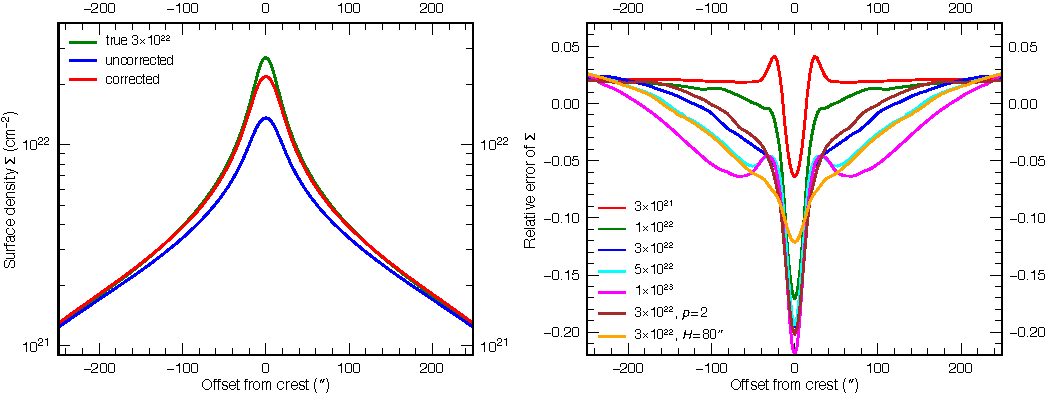
\includegraphics[width=0.97\textwidth]{fig_cylinders.pdf}
\caption{The isolated radiative transfer cylinders reconstructed by \emph{hires} at $O = 13.5{\arcsec}$ and corrected. \emph{Left}: the
profile across the cylinder with $3{\times}10^{22}$\,cm$^{-2}$ on its axis, true (convolved to the beam), uncorrected and
corrected. \emph{Right}: relative error of the corrected surface density across all seven cylinders, labeled by their surface
density on the axis. Each profile is the median over the middle part of the cylinder.}
\label{fig:cylinders}
\end{figure*}

Without the correction, the crests of the filaments are too low by $14$\% for the least dense filament and by $58$\% for the
densest, and the profiles are too wide and too shallow, because the crest is suppressed much more than the wings. After the
correction, the linear densities are within $7$\% of the truth and the slopes of the profiles within $0.05$. The crests remain $6$
to $22$\% too low, and the widths of the six filaments with $H = 48{\arcsec}$ at $O = 13.5{\arcsec}$ (intrinsic $H = 40{\arcsec}$)
are $15$ to $31$\% too large, because the axis of a filament, like the center of a core, is colder than the middle of a uniform
structure with the same surface density. Beyond about $20{\arcsec}$ from the crest, the corrected profiles are within $8$\% of the
truth.

\subsection{Simulated sky}
\label{sec:sim}

The models of Sects.~\ref{sec:valgrid} and \ref{sec:cyl} each contain a single structure. An observed field does not. The simulated
sky of Sect.~\ref{sec:modcloud} contains a cloud, seven filaments and $96$ cores, which overlap along the lines of sight.

\begin{figure*}
\centering
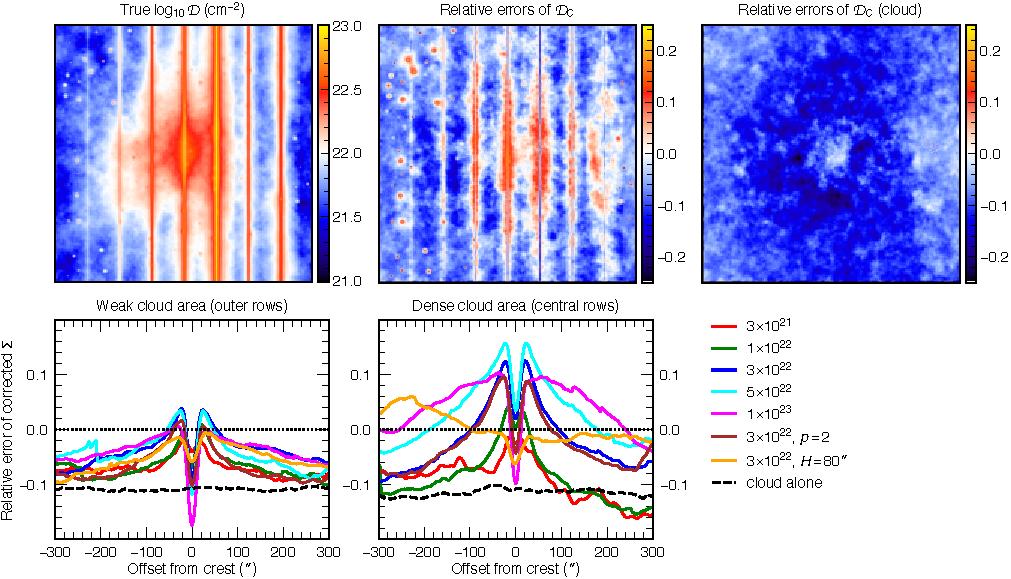
\includegraphics[width=\textwidth]{fig_simsky6.pdf}
\caption{The simulated sky, built from radiative transfer models of a cloud, seven filaments and $96$ cores. \emph{Upper left}: the
true surface density at $O = 13.5{\arcsec}$. \emph{Upper middle}: the relative error of the corrected surface density, (corrected $-$
true) / true. \emph{Upper right}: the same for a sky that contains the cloud alone. \emph{Lower panels}: the relative error
across each filament, as the median over the outer rows of the field, where the cloud is weak, and over its central rows, where
the cloud is dense. The filaments are labeled by their surface density on the axis. The cores are masked in the profiles. The
dashed curve is the cloud alone at the same positions.}
\label{fig:simsky6}
\end{figure*}

%%%%% -----------------------------------------------------------------------------------------------------------------------------
%%%%% NUMBERS (2026-10-20): Sect. 5.3 from python/paper_numbers/simsky_numbers.py on simsky6_RT_enh_cirrdepth=2_nocrater (the sky),
%%%%% simsky6_RT_enh_cirronly (the cloud alone) and the core catalog simsky6.w40.cores.cores.txt. The crests, flanks and wings are
%%%%% read from the profiles at 0, 15-45 and 240 arcsec; the total of 0.96 is the median accuracy ratio with the cores masked
%%%%% (0.955).
%%%%% -----------------------------------------------------------------------------------------------------------------------------
Figure~\ref{fig:simsky6} shows the result for each component. The cloud alone, in a sky without filaments and cores, is corrected
from $0.76$ to $0.89$ of the truth in the median. It is $6$\% too low at $10^{21}$\,cm$^{-2}$ and $14$\% too low at
$10^{22}$\,cm$^{-2}$. The remaining underestimation of $\Sigma$ in the cloud is the price of the average of
Sect.~\ref{sec:diffuse}, which gives half the weight to the sphere.

In the outer parts of the field, the cloud is a few $10^{21}$\,cm$^{-2}$. There the crests of the filaments are corrected to within
$4$ to $17$\%, and their flanks to within $5$\%. Their outer wings are corrected too little, by $6$ to $9$\%, as much as the cloud
around them. In the center of the field, the cloud reaches $2$ to $3\times10^{22}$\,cm$^{-2}$. There the flanks of the dense
filaments are corrected too much, by $10$ to $16$\%, while the cloud alone at the same positions is corrected too little. Both
effects come from the superposition of two structures, which a correction based on the surface density alone treats as one. They
have the signs predicted in Appendix~\ref{app:arrange}: a structure in a weak cloud is under-corrected, and a structure in a dense
cloud is over-corrected. The central cloud of the simulated sky is two to three times denser than the background of the filaments
in Aquila, which \emph{getsf} finds to be $6$ to $10\times10^{21}$\,cm$^{-2}$ at most. In a field like Aquila, the over-correction
of the flanks should therefore be about $10$\%. Over the whole field, with the cores masked, the corrected surface density is
$0.96$ of the truth.

\subsection{Remaining errors}
\label{sec:base}

%%%%% -----------------------------------------------------------------------------------------------------------------------------
%%%%% NUMBERS (2026-10-20): from validate3_finRTlaw.txt.nodes.txt (validate_calib3.py, per node), the 926 nodes with a half radius
%%%%% r_h below 13.5 arcsec, row 'hicorrect2, fine': median and 16th percentile of the central residual, median and 84th percentile
%%%%% of the largest residual of the radial profile within 3 r_h.
%%%%% -----------------------------------------------------------------------------------------------------------------------------
Two kinds of structure are not corrected well by any correction that depends on the surface density alone. The centers of
concentrated structures, the centers of cores and the crests of filaments, remain $6$ to $22$\% too low. Cores narrower than $2\,O$,
half of the models of the grid, remain $27$\% too low at their centers in the median and more than $56$\% too low for $16$\% of them.
They are surrounded by a ring that is over-corrected by $5$\% in the median and, for $16$\% of them, by more than $16$\%, because
the beam spreads their cold centers over an area of lower surface density. Superposed structures of very different temperatures are
corrected too little or too much, by $10$ to $20$\% (Sect.~\ref{sec:sim}). Corrections that also read the fitted temperature do not
help (Appendix~\ref{app:tcorr}).

% =====================================================================

\section{Application to the Aquila cloud}
\label{sec:aquila}

The correction was applied to a $31\arcmin \times 31\arcmin$ sub-field of the Aquila cloud (centered at RA $277{\fdg}4765227$, Dec
$-1{\fdg}9962943$). The field was observed with \emph{Herschel} \citep{Andre+2010, Konyves+2015}. The reconstruction used the
images at $160$, $250$, $350$, and $500${\um}. The field contains $625\times 625$ pixels of $3{\arcsec}$. The factor was evaluated
on the reconstruction at $O = 13.5{\arcsec}$ and applied to it. Every pixel was corrected, including those toward protostars
(Appendix~\ref{sec:notdo}).

The radiation field of the cloud was estimated with the procedure of Appendix~\ref{app:fieldest}, from the diffuse material of the
whole Aquila map, which contains $29$ million pixels. The field is $G_0 \approx 33$, with $25$ and $41$ for the 16th and 84th
percentiles of the temperature. The correction therefore used $G_0 = 33$ in Eq.~(\ref{eq:factorg0}), about three times the field of
the calibration.

%%%%% -----------------------------------------------------------------------------------------------------------------------------
%%%%% NUMBERS (2026-10-20): Sect. 6 from python/paper_numbers/aquila_numbers.py on the images of hires/Aquila_cutout_g33
%%%%% (hicorrect2 with -g0=33); the values for G_0 = 10 are recomputed by the same script from hicorrect2.py.
%%%%% -----------------------------------------------------------------------------------------------------------------------------
The median correction factor over the field is $1.70$. It lies between $1.21$ and $2.10$ for $98$\% of the pixels and reaches its
maximum of $2.10$ near $3{\times}10^{22}$\,cm$^{-2}$, so the correction is significant everywhere in the field. The total surface
density of the field increases by a factor of $1.86$. With the calibration field $G_0 = 10$, the median factor would be about
$1.45$ and the total would increase by a factor of about $1.61$.

The distribution of surface densities changes more than the median factor suggests, because the factor rises with the surface
density. The median surface density of the field increases from $9.7{\times}10^{21}$ to $1.7{\times}10^{22}$\,cm$^{-2}$, and its
99th percentile from $5.6{\times}10^{22}$ to $1.1{\times}10^{23}$\,cm$^{-2}$. The numbers of pixels above $10^{22}$,
$3{\times}10^{22}$ and $10^{23}$\,cm$^{-2}$ increase by factors of $1.8$, $5.2$ and $8.1$. This matters for any criterion based on
a surface density threshold, such as that for star formation.

The corrected surface density implies a lower dust temperature. It was defined as the temperature at which the corrected surface
density gives the same intensity at $500${\um} as the uncorrected surface density with the fitted temperature. Its median over the
field is $12.2$\,K, against $15.0$\,K for the fitted temperature. It is below $9.6$ and $18.6$\,K for $1$ and $99$\% of the pixels.

\begin{figure*}
\centering
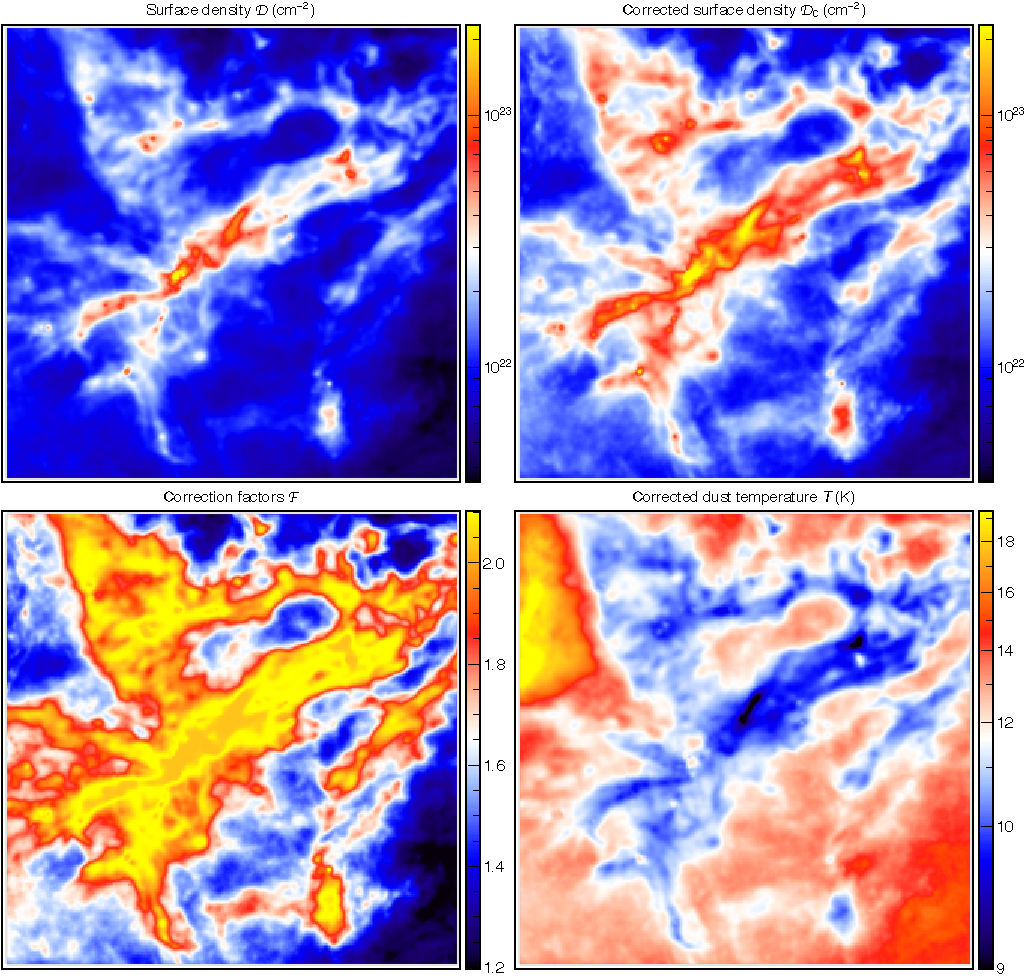
\includegraphics[width=\textwidth]{fig_aquila.pdf}
\caption{The Aquila field at $O = 13.5{\arcsec}$, corrected for the field $G_0 = 33$. \emph{Upper panels}: the surface density before
and after the correction, on a common logarithmic scale. \emph{Lower panels}: the image of the correction factors $\mathcal{F}$ and
the corrected dust temperature (Sect.~\ref{sec:aquila}). }
\label{fig:aquila}
\end{figure*}

Figure~\ref{fig:aquila} shows the field before and after the correction, together with $\mathcal{F}$ and the corrected dust
temperature. The correction is not a uniform rescaling. The factor is smallest in the diffuse material between the structures and
largest along the crests of the filaments and at the cores. The correction therefore raises the contrast of the image as well as
its overall level. Above $3{\times}10^{22}$\,cm$^{-2}$, the factor changes by only a few percent, so the densest crests and cores receive nearly
the largest correction, and the corrected temperature shows no artificial dips toward them. The field is not uniform across the cloud. The warm
corner at the upper left of the temperature map is heated more strongly than the rest of the field, and there the single field of
the cloud underestimates the true one. Appendix~\ref{sec:field} discusses the uncertainty due to the radiation field.

\section{Conclusions}
\label{sec:conclusions}
% NUMBERS: the values of the conclusions are copied from Sects. 3.2, 5, 6 and 7; see the comments there.

Surface density images of molecular clouds are derived by fitting one modified blackbody to each pixel. These images are
systematically too low wherever the dust temperature varies along the line of sight. The underestimation exceeds a factor of two in
the densest material. It cannot be measured from the observed colors, because its signature of $1$ to $6$\% of the intensities
would amplify the photometric errors $7$ to $9$ times. The correction must therefore come from radiative transfer.

Radiative transfer provides a single relation between the dust temperature and the effective column $\Sigma_{\rm A}$ that shields
the dust. It describes $2086$ models of embedded Bonnor--Ebert spheres and seven models of filaments, with a scatter of $2.4$\%. A
sphere, a cylinder and a plane-parallel layer of the same surface density need factors within $10$\% of each other. The relation
gives the correction factor $f$ as an explicit function of the observed surface density. At low surface densities, the factor is
calibrated on a radiative transfer model of an extended cloud, whose warm surface layers the relation does not describe.

The correction applies to a conventional surface density map at the resolution of the longest waveband and to the higher-resolution
images of the \emph{hires} reconstruction. The factor was evaluated on the finest image, which gives the sharpest corrected images
and the most accurate masses.

The correction was tested on three kinds of radiative transfer models. On $1815$ models of cores that were not used in the
calibration, it raises the median core mass from $0.63$ to $0.98$ of the true mass and the total surface density from $0.78$ to
$0.99$. On seven isolated filaments, it restores the linear densities to $0.93$--$1.01$ of the truth and the slopes of the profiles
to within $0.05$. On a simulated sky of cloud, filaments and cores, all computed with radiative transfer, it restores the total
surface density to $0.96$. The centers of cores and the crests of filaments remain $6$ to $22$\% too low, because they are colder
than a uniform structure with the same surface density. Structures superposed on a cloud are corrected too little where the cloud
is weak and too much where it is dense, by about $10$\% in a cloud like Aquila.

The correction leaves only a few percent in the median core mass, less than the error of a footprint wrong by a quarter of its
radius ($-15$ to $+8$\%). A correction that depends on the surface density alone is therefore sufficient. Corrections that also use
the fitted temperature are not worth their complexity, because a warm pixel may need either more or less correction.

The correction was calibrated for $G_0 = 10$. Models computed for nine fields from $G_0 = 1$ to $483$ show that, without further
adjustment, it is too large by up to $27$\% in the weakest fields and too small by up to $20$\%
in fields of $G_0 \approx 20$--$100$. A
field factor measured on these models, a function of the surface density and the field, brings these errors to within $4$\% of
those in the calibration field, and to within $6$\% for fields left out of its construction. The field of a cloud, estimated from
the temperatures of its diffuse material, ranges from below $1$ (Taurus) to about $250$ (Cygnus~X) in nine regions. The other main
uncertainty is the floor temperature $T_{\rm min}$ of fully shielded dust, to which $f$ is very sensitive above
$10^{22}$\,cm$^{-2}$.

Applied to a field of the Aquila cloud, whose diffuse material requires $G_0 \approx 33$, the correction raises the total surface
density by a factor of $1.86$ and the number of pixels above $10^{23}$\,cm$^{-2}$ by a factor of $8.1$. The median dust
temperature implied by the corrected surface densities is $12.2$\,K, against $15.0$\,K for the fitted one.

For the adopted dust properties, the total uncertainties of corrected surface densities are about $30$\% in diffuse material and
$50$\% in dense structures, and those of corrected temperatures about $2$\,K (Appendix~\ref{sec:accuracy}). The dust opacity adds a
factor of about $1.5$ to $2$.

\begin{acknowledgements}
The images of the molecular clouds used in this work were downloaded from the \textit{Herschel} Science
Archive\footnote{\url{http://archives.esac.esa.int/hsa/whsa/}} and processed with the \emph{hires} method
\citep{Menshchikov2021method} by Guo-Yin Zhang. The images were obtained in the \textit{Herschel} Gould Belt Survey
(HGBS\footnote{\url{http://gouldbelt-herschel.cea.fr}}) (PI: Ph.\,Andr{\'e}), HOBYS\footnote{\url{http://hobys-herschel.cea.fr}}
(PI: F.\,Motte, A.\,Zavagno, S.\,Bontemps), and A-CMC (PI: P.\,Harvey) projects. HGBS and HOBYS are the \textit{Herschel} Key
Projects jointly carried out by SPIRE Specialist Astronomy Group 3 (SAG3), scientists of several institutes in the PACS Consortium
(e.g., CEA Saclay, INAF-IAPS Rome, LAM/OAMP Marseille), and scientists of the \textit{Herschel} Science Center (HSC).
\end{acknowledgements}

\bibliographystyle{aa}
\bibliography{hires2_correction}

% =====================================================================

\appendix
\nolinenumbers

\section{Details of the radiative transfer models}
\label{app:rtmodels}

\subsection{Grids of core models}
\label{sec:grid}

All models of cores were Bonnor--Ebert spheres embedded in a uniform spherical cloud, heated from outside by the interstellar
radiation field and computed with \emph{radmc-3d} for the dust of Sect.~\ref{sec:models}. Three grids were used: the main grid for
the relation of Eq.~(\ref{eq:law}), the subdivision grid for the validation of Sect.~\ref{sec:valgrid}, and the grid of radiation
fields for Appendix~\ref{app:field}.

The main grid varied three parameters: the surface density $\Sigma_{\rm emb}$ of the embedding cloud, from $3.75\times10^{20}$ to
$9.6\times10^{22}$\,cm$^{-2}$ in $9$ steps of a factor of $2$; the mass of the Bonnor--Ebert sphere, from $1.6{\times}10^{-3}$ to
$31\,M_{\odot}$ in $26$ steps of $0.17$\,dex; and the half-maximum width of its volume density profile, from $0.003$ to $0.25$\,pc
in $19$ steps of $0.11$\,dex. Only the models whose peak surface density exceeded that of the embedding cloud by at least $5$\%
were computed, and one of them, the most extended one, was not completed because it required too much memory. The central-to-edge
density ratios $\rho_{\rm C}/\rho_{\rm e}$ of the $2086$ computed models ranged from $1.04$ to $2.1{\times}10^{3}$. Three more
models extended the grid to $\Sigma_{\rm emb}$ of $1.9$ to $7.9\times10^{23}$\,cm$^{-2}$. They were optically thick in the far
infrared and were not used in the calibration (Sect.~\ref{sec:modcores}). The temperature of each model, tabulated shell by shell,
entered the relation of Eq.~(\ref{eq:law}).

The attenuating columns of Eq.~(\ref{eq:seff}) were computed by integrating the density along rays. For the spherical shells of the
cores, a direction is defined by its angle $\psi$ to the outward radial direction, and $240$ values of $\psi$ were used, weighted
by $\sin\psi$. Each filament was treated as an infinite cylinder with the same profile. A direction is then defined by its angle
$\theta$ to the axis and by the angle $\phi$ between its projection onto the cross-section and the outward radial direction. The
$200$ values of $\cos\theta$ and the $180$ values of $\phi$ were spaced uniformly, so that all directions represent equal solid
angles. Few photon packets of the Monte Carlo calculation arrived near the centers of the densest cores, and the temperatures of
their innermost shells scattered widely. A shell among the ten innermost ones was rejected if its temperature differed by more than
$10$\% from the median of its five neighbors, together with every shell inside it. The rejected shells were $1.8$\% of all shells
and contained a negligible fraction of the mass, and the fit does not depend on this choice. The outermost shell of every sphere
was also rejected. In the thicker embedding clouds, it spans an extinction of several magnitudes, and its single Monte Carlo
temperature, an average over a steep temperature gradient, exceeded that of the dust at its center, where $\Sigma_{\rm A}$ was
evaluated, by up to $2.4$\,K.

The models of the subdivision grid lay between the models of the main grid and were not used in the relation. The footprint of a
model is the area of its convolved true image that stands above the embedding cloud. Its background is the median surface density
in a ring $15{\arcsec}$ wide just outside the footprint. For $65$ models, the mass of the core could not be measured: the ring
contains fewer than $20$ valid pixels, because the footprint reaches the edge of the image, or the true mass within the footprint
is not positive, because the core barely stands above its cloud.

The grid of radiation fields repeated $305$ models of the main grid, together with $34$ models at a tenth embedding surface density
of $1.92\times10^{23}$\,cm$^{-2}$. They were computed for nine strengths of the radiation field, from $G_0 = 0.98$ to $483$, in
steps of a factor of $2.17$. The lowest field is the field of \citet{Black1994} alone, without the hot component, and no weaker
field is possible in this implementation. About five models per field were not computed, because they required the largest images.
They do not affect the results of Appendix~\ref{app:field}.

\subsection{Computing the isolated cylinders}

The cylinders were computed with \emph{radmc-3d} on an axisymmetric spherical grid of $400$ cells in radius and $480$ cells in the
polar angle, which covered both sides of the equatorial plane. The grid was refined toward the axis and toward the equatorial
plane. The temperatures of the Monte Carlo calculation were averaged over the middle part of the cylinder, in bins of the distance
$r$ from the axis, which removed most of the Monte Carlo noise. The isolated cylinders were computed with $2\times10^9$ photon
packets. The parameters of the eight cylinders are listed in Table~\ref{tab:cylpar}. The width $h$ of each model was chosen to give
the required $H$ (Table~\ref{tab:cylpar}).

\begin{table}[ht!]
\caption{The cylinders of Sect.~\ref{sec:modfil}. $\Sigma_0$: the surface density on the axis. $p$ and $h$: the slope and the
half-maximum width of the volume density profile of Eq.~(\ref{eq:fdens}). $H$: the half-maximum width of the surface density
profile. The densest cylinder was optically thick and was not used.}
\label{tab:cylpar}
\centering
\begin{tabular}{lccc}
\hline\hline
\noalign{\smallskip}
$\Sigma_0$ (cm$^{-2}$) & $p$ & $h$ (${\arcsec}$) & $H$ (${\arcsec}$) \\
\noalign{\smallskip}
\hline
\noalign{\smallskip}
$3{\times}10^{21}$ & $1.75$ & $20.3$ & $40$ \\
$1{\times}10^{22}$ & $1.75$ & $20.3$ & $40$ \\
$3{\times}10^{22}$ & $1.75$ & $20.3$ & $40$ \\
$5{\times}10^{22}$ & $1.75$ & $20.3$ & $40$ \\
$1{\times}10^{23}$ & $1.75$ & $20.3$ & $40$ \\
$2{\times}10^{23}$ & $1.75$ & $20.3$ & $40$ \\
$3{\times}10^{22}$ & $2$    & $23.7$ & $40$ \\
$3{\times}10^{22}$ & $1.75$ & $42.5$ & $80$ \\
\noalign{\smallskip}
\hline
\end{tabular}
\end{table}

The mirror symmetry of \emph{radmc-3d} was not used. On a test sphere, it made the temperatures $0.6$ to $1.1$\,K too low, whereas
the full grid agreed with a one-dimensional calculation to $0.15$\,K.

\subsection{Cylindrical envelopes for the simulated sky}
\label{app:embfil}

The filaments of the simulated sky were the cylinders of Sect.~\ref{sec:modfil}, each computed again inside a cylindrical envelope
that stood for the cloud around it. The envelope was uniform in radius between $R = 0.5$\,pc and $1$\,pc, and the cylinder was
$10.3$\,pc long, longer than the field, so that its ends lay outside the images. The surface density of the envelope through the
axis followed the cloud of the sky along the filament, row by row. A cylindrical envelope shields the axis less than a cloud layer
of the same surface density, because the layer also blocks the directions close to its plane. The envelope was therefore made $1.3$
to $1.6$ times denser than the cloud, so that the mean intensity at the axis was the same as in the middle of the cloud layer. The
temperatures were averaged in a running window $0.2$\,pc long along the axis, which followed the variation of the envelope. Each
model was imaged twice: once in full, and once with the volume of the filament emptied while all temperatures were kept. The
difference is the emission of the filament inside the cloud, without the emission of the envelope itself. It was added to the cloud
of the sky, which was assumed to extend far in front of and behind the filament. The embedded filaments were computed with $10^9$
photon packets. Runs with $8\times10^9$ packets gave the same temperatures to $0.02$\,K and the same emission to $0.3$\%.

\subsection{Three-dimensional model of the diffuse cloud}

The cloud of the simulated sky was a three-dimensional radiative transfer model whose projection is the map of the cloud. A surface
density map does not determine the density along the line of sight, and the model is one of the many distributions that project to
the map. The map had scale-free fluctuations, with a power spectrum $P(k) \propto k^{-3.0}$, a median surface density of about
$3{\times}10^{21}$\,cm$^{-2}$, and no large-scale gradient. Real clouds such as Aquila have an extended background that rises
toward their centers. The map was therefore multiplied by $1 + 5\,[1 + (r/600{\arcsec})^2]^{-0.75}$, where $r$ is the distance from
the center of the field. This factor is $6$ at the center, nearly constant within $600{\arcsec}$, and declines as $r^{-1.5}$
beyond, toward unity far from the center, while the fine structure of the map is kept. The same enhanced map was used for the cloud
of the simulated sky and for the envelopes of the embedded filaments. The map was averaged into cells of $12{\arcsec}$ and extended
on every side by margins of $2$\,pc, by mirror reflection. The margins kept the heating through the sides of the box away from the
field.

The volume density was built in three steps. First, a Gaussian random field $G$ of unit variance, with the same power spectrum
$P(k) \propto k^{-3.0}$ in three dimensions, filled a box with the area of the extended map and a depth of $2$\,pc. Second, its
log-normal transform $g = \exp(s\,G - s^2/2)$, with the amplitude $s = 0.5$, gave positive fluctuations with a mean of unity and a
root-mean-square contrast of about $50$\%. Third, every column of $g$ was rescaled so that its integral equaled the surface density
of the map in that pixel, $n(x, y, z) = \Sigma(x, y)\,g(x, y, z) / \int g\,{\rm d}z$. The projection of the box is therefore
exactly the map, while the density varies along every line of sight as it does across the sky. With the margins, the box had $712
\times 712 \times 132$ cells ($10.8 \times 10.8 \times 2.0$\,pc) and was computed with $8\times10^{10}$ photon packets. Fewer
photon packets, cells of $24{\arcsec}$, or a box without fluctuations along the line of sight gave the same correction factors to
$0.1$\%.

Figure~\ref{fig:cube} shows a slice through it, along one row of the field and
the line of sight, and compares it with the analytic slab of the same surface density. The surface layers are up to $3$\,K warmer
than the slab, because they are heated by the unattenuated ultraviolet radiation from half the sky, which the gray relation of
Eq.~(\ref{eq:law}) does not describe. Thin columns between dense regions are up to $2$\,K colder than the slab, because their dense
neighbors shield them from the side.

\begin{figure*}[ht!]
\centering
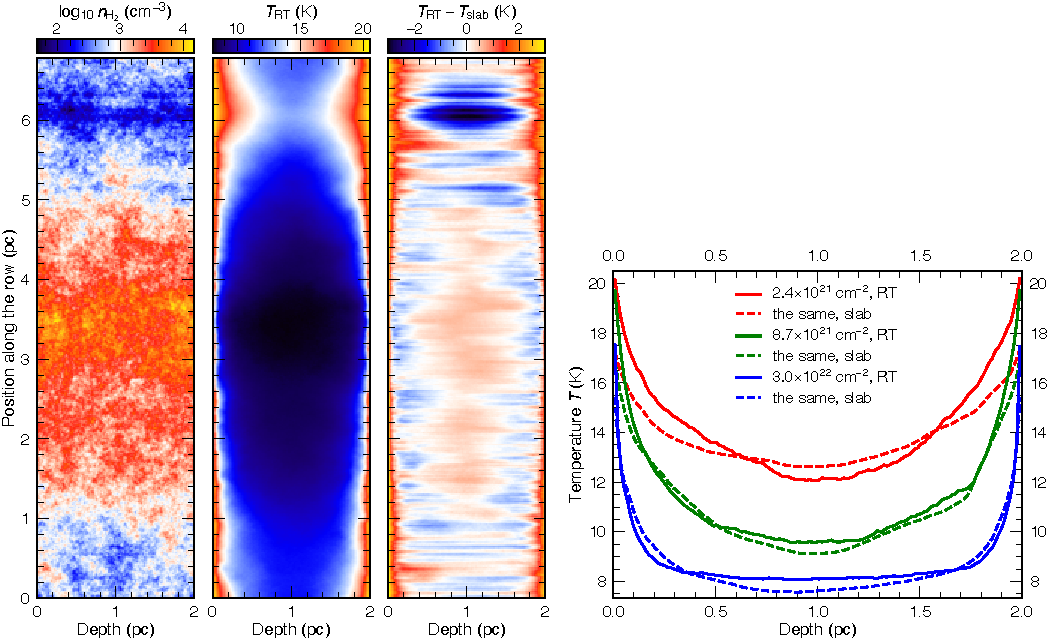
\includegraphics[width=0.9\textwidth]{fig_cube.pdf}
\caption{A slice through the radiative transfer model of the cloud, along the middle row of the field (vertical axis) and the line
of sight (horizontal axis). The depth along the line of sight is horizontal in all four panels. \emph{Left three panels}: the H$_2$
number density, the dust temperature, and the difference between the dust temperature and that of the analytic slab with the same
surface density in each column. \emph{Right panel}: the dust temperature against the depth for three columns of different surface
density, in the radiative transfer model (solid) and in the analytic slab (dashed).}
\label{fig:cube}
\end{figure*}

As a result, the emission of the radiative transfer model at $160${\um} is up to $1.5$ times that of the analytic slab with the same
surface density. In the simulated sky, the emission of the analytic slab was multiplied in each band by the ratio of the emission of
the radiative transfer model to that of the slab, computed in each cell and interpolated to the pixels. The sky thus had the
temperatures of the radiative transfer model and the fine structure of the map of the cloud.

\section{The arrangement of the material along the line of sight}
\label{app:arrange}

The correction is applied pixel by pixel. A pixel receives the emission of everything along its line of sight, and a single
modified blackbody is fitted to this sum. The fit is therefore biased by the whole distribution of dust temperatures along the line
of sight, not by the temperature of any one structure. The method replaces this distribution by the one of a single uniform body
with the same total surface density. This appendix explains why a sphere and a layer are the limiting shapes and measures the error
of this replacement. In a plane-parallel geometry, the emergent emission depends only on the total surface density
(Sect.~\ref{sec:orient}).

\subsection{A sphere and a layer as limiting cases}
\label{app:shape}

\begin{figure*}[ht!]
\centering
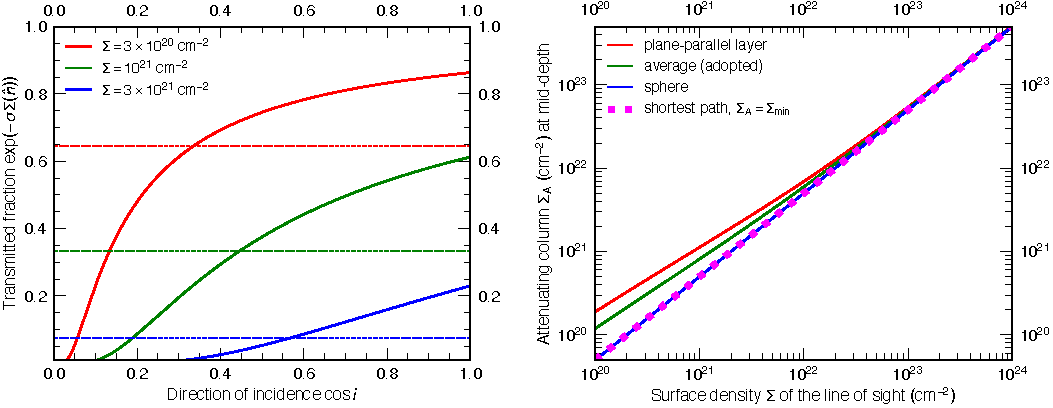
\includegraphics[width=0.96\textwidth]{fig_angular.pdf}
\caption{\emph{Left}: The fraction of the heating radiation that survives the journey inward, against the direction it comes from,
for a dust grain at mid-depth of a plane-parallel layer of three total surface densities. Plotted against the cosine of the angle,
the angular mean of each curve is the area beneath it, drawn dashed; the single column that would produce that same mean intensity
is the effective attenuating column of Eq.~(\ref{eq:seff}). \emph{Right}: that column against the total surface density of the line
of sight, for the two limiting shapes and for the average of them that is adopted, with the shortest path $\Sigma_{\rm min}$ for
comparison.}
\label{fig:angular}
\end{figure*}

The cylinder in Fig.~\ref{fig:relation} shows that the sphere and the layer are indeed the limits. A cylinder is bounded across its
axis, like a sphere, and unbounded along it, like a layer. Its factor lies between them at every surface density, within $5$\% of
the sphere and within $6$\% of the layer. The layer is an extreme case because it is unbounded across the line of sight. For a
grain at the midplane, the path to the boundary is the half-thickness divided by the cosine of the angle to the normal. This path
diverges as the angle approaches $90\degr$, so a whole band of directions near the plane of the layer delivers no radiation,
however thin the layer is. At $10^{22}$\,cm$^{-2}$, the directions within $30\degr$ of the normal deliver $64$\% of the mean
intensity, and those within $45\degr$ deliver $93$\%. In a bounded body, the path is finite in every direction, and no direction is
lost. The sphere is the opposite extreme: a compact body with a given central surface density blocks less of the sky than any other
body with that surface density. Every real cloud lies between the two limits, and the range between them is the full effect of the
shape. This is why the method needs no assumption about the shape of a cloud.

The dotted curve of Fig.~\ref{fig:relation} shows what happens if $\Sigma_{\rm A}$ is replaced by $\Sigma_{\rm min}$
(Sect.~\ref{sec:why}), so that each dust grain is heated only through its least shielded direction. This makes the material near
the surfaces too warm while leaving the interior almost unchanged. It maximizes the spread of temperatures along the line of sight,
and with it the required correction.

Along a central line of sight, $\Sigma_{\rm min} = \min(u, 1-u)\,\Sigma$ (Fig.~\ref{fig:geometry}), which rises linearly from zero
at either surface to $\Sigma/2$ at the midplane, so that its average over the depth is $\Sigma/4$. Below
$3{\times}10^{21}$\,cm$^{-2}$, this simpler treatment agrees with the full calculation to $2$\%. Above $10^{22}$\,cm$^{-2}$ it
diverges, and at $10^{23}$\,cm$^{-2}$ it overestimates the correction by half. At high surface densities this curve also declines,
for the same reason as the curves of the uniform bodies (Sect.~\ref{sec:factor}).

\subsection{Centrally concentrated structures}
\label{app:concentr}

In the plane-parallel limit, the density profile has no effect at all. Concentration can therefore act only through the radiation
that reaches the dust from the sides. A bounded structure allows this, and a layer does not. The effect was measured on a sphere
with the density $\rho(r) \propto (1 + r^2/a^2)^{-1}$ out to its boundary. The sphere was normalized so that the column through its
center equaled the observed one, and $a$ was set by the central-to-edge density ratio. The positions along the central line of
sight were weighted by the density there, as in the emission. For each position, the column was integrated along the ray to the
boundary in every direction of the average.

\begin{table}[ht!]
%%%%% -----------------------------------------------------------------------------------------------------------------------------
%%%%% NUMBERS (2026-10-20): Table tab:concentr, and the numbers of Appendix B on two components,
%%%%% from python/paper_numbers/superposition_numbers.py, which uses superposition_test.py and hicorrect2.py.
%%%%% -----------------------------------------------------------------------------------------------------------------------------
\caption{Correction factor required by the central line of sight of a sphere of the given central surface density, for four
central-to-edge density ratios. The first column is a uniform sphere.}
\label{tab:concentr}
\centering
\begin{tabular}{lcccc}
\hline\hline
\noalign{\smallskip}
$\Sigma$ (cm$^{-2}$) & uniform & $10$ & $10^2$ & $10^3$ \\
\noalign{\smallskip}
\hline
\noalign{\smallskip}
$5{\times}10^{21}$ & $1.093$ & $1.133$ & $1.169$ & $1.189$ \\
$1{\times}10^{22}$ & $1.276$ & $1.335$ & $1.409$ & $1.460$ \\
$3{\times}10^{22}$ & $1.699$ & $1.756$ & $1.892$ & $2.039$ \\
$1{\times}10^{23}$ & $1.835$ & $1.881$ & $1.981$ & $2.165$ \\
\noalign{\smallskip}
\hline
\end{tabular}
\end{table}

Table~\ref{tab:concentr} gives the result. Concentration always raises the required correction, because the mass of a concentrated
structure lies where the shielding is deepest. The effect is $2$ to $5$\% for a density ratio of $10$ and $9$ to $20$\% for a ratio
of $10^3$. It is one-sided. A correction built on uniform structures therefore under-corrects a concentrated structure and never
over-corrects it.

\subsection{Two superposed components}
\label{app:twocomp}

The second case is a line of sight that crosses a cloud with a denser structure embedded in it at an unknown depth. The model
consisted of a plane-parallel cloud of surface density $\Sigma_{\rm cl}$. The material at the column depth $x$ in the cloud is
shielded by the angular average of $x/|\mu|$ toward the observer and of $(\Sigma_{\rm cl} - x)/|\mu|$ away from the observer. A
uniform sphere with the surface density $\Sigma_{\rm s}$ through its center is embedded in the cloud. A fraction $q$ of the cloud
lies in front of the sphere. A dust grain at the signed position $z$ along the diameter of the sphere, in units of its radius, is
shielded by its own sphere over the path
\begin{equation}
   l(z,\psi) = -z\cos\psi + \left(1 - z^2\sin^2\psi\right)^{1/2},
\label{eq:lsphere}
\end{equation}
in units of the radius. It is also shielded by the cloud over $q\,\Sigma_{\rm cl}/|\cos\psi|$ toward the observer and
$(1-q)\,\Sigma_{\rm cl}/|\cos\psi|$ away from the observer. The angular average of Eq.~(\ref{eq:seff}) was taken over $\psi$ with
the isotropic weight $\sin\psi$, and the temperature of every grain followed from Eq.~(\ref{eq:law}). The emissions of the cloud
and of the sphere were added with their masses, and one modified blackbody was fitted to the sum, exactly as in the reconstruction.
This gave the fitted surface density $\Sigma_{\rm F}$ of the composite line of sight and the factor $\Sigma/\Sigma_{\rm F}$ that it
requires. The method sees only $\Sigma_{\rm F}$ and applies $f(\Sigma_{\rm F})$ of Eq.~(\ref{eq:factor}). The error of the
corrected surface density is therefore $f(\Sigma_{\rm F})\,\Sigma_{\rm F}/\Sigma - 1$.

\begin{figure*}[ht!]
\centering
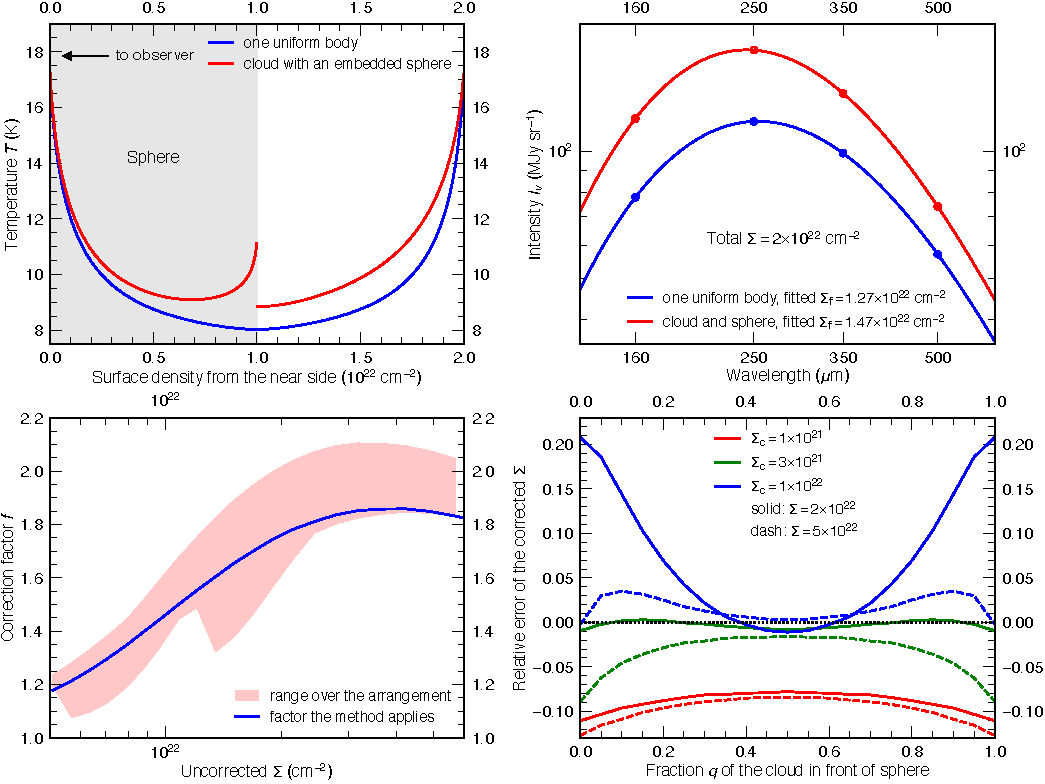
\includegraphics[width=0.95\textwidth]{fig_superposition.pdf}
\caption{Superposition of a cloud and a sphere. \emph{Upper left}: The dust temperature along a line of sight of
$2{\times}10^{22}$\,cm$^{-2}$. One curve is for the uniform body that the method assumes. The other curve is for the same surface
density divided equally between a cloud and a uniform sphere at the near side of the cloud ($q = 0$). \emph{Upper right}: The
emission of the two lines of sight, with the surface density $\Sigma_{\rm F}$ that a single modified blackbody fit returns. The two
lines of sight have the same true surface density. \emph{Lower left}: The factor that the method applies and the range of factors
that the composite lines of sight require, both against the observed (fitted) surface density. The range covers cloud surface
densities $\Sigma_{\rm cl}$ of $10^{21}$, $3{\times}10^{21}$ and $10^{22}$\,cm$^{-2}$ and all positions of the sphere. \emph{Lower
right}: Relative error of the corrected surface density against the fraction $q$ of the cloud in front of the sphere. Colors give
the surface density of the cloud $\Sigma_{\rm cl}$; solid and dashed curves are for total surface densities of $2{\times}10^{22}$
and $5{\times}10^{22}$\,cm$^{-2}$.}
\label{fig:superposition}
\end{figure*}

%%%%% -----------------------------------------------------------------------------------------------------------------------------
%%%%% NUMBERS (2026-10-20): from python/paper_numbers/superposition_numbers.py (range of the error over q; the worked example:
%%%%% q = 0, Sigma = 2e22, Sigma_cl = 1e22 cm^-2).
%%%%% -----------------------------------------------------------------------------------------------------------------------------
Figure~\ref{fig:superposition} gives the result. The error of the corrected surface density ranges from $-13$ to $+21$\%. Its sign
depends on the cloud. A weak cloud ($\Sigma_{\rm cl} = 10^{21}$\,cm$^{-2}$) leaves the sphere nearly isolated. The sphere needs
more correction than the average of a sphere and a layer, so the correction is too small by $8$ to $13$\%, at any depth. A dense
cloud ($\Sigma_{\rm cl} = 10^{22}$\,cm$^{-2}$) with the sphere at one of its sides makes the line of sight warmer than a single
body. The correction is then too large, by up to $21$\%. When the sphere lies near the middle of a dense cloud, the error is only a
few percent. The simulated sky of Sect.~\ref{sec:sim}, built entirely from radiative transfer models, shows both regimes: the wings
of filaments in its weak outer cloud are corrected too little, and the flanks of filaments in its dense central cloud too much.

The upper panels of Fig.~\ref{fig:superposition} show why the effect exists. A sphere at the near side of the cloud loses radiation
sideways, and nothing in front of it blocks the incoming radiation. This line of sight is warmer and brighter than the uniform body
of the same surface density, and the fit returns $1.47{\times}10^{22}$ instead of $1.27{\times}10^{22}$\,cm$^{-2}$. The method then
applies the factor of a uniform body with this observed surface density, $1.64$ instead of the required $1.36$, and the corrected
surface density is $21$\% too high. Nothing observable distinguishes the two lines of sight, so this error is an irreducible
uncertainty of any method of this kind.

\section{Calibration for different radiation fields}
\label{app:field}

The relation of Eq.~(\ref{eq:law}) was measured for a single field, $G_0 = 10$. A stronger field heats the dust at every
attenuating column, and this changes the underestimation of $\Sigma$ by the fit. To measure the effect, the correction was tested
on the grid of radiation fields of Appendix~\ref{sec:grid}, comparing for every pixel the factor that restores its true surface
density with the factor that the correction applies. The first column of Table~\ref{tab:fieldR} gives the relative error of the
corrected surface density without the field factor. The error changes sign twice: the correction is too large in the weakest
fields, too small for $G_0 \approx 20$--$100$, and again too large at the highest surface densities in the strongest fields. The
underestimation of $\Sigma$ by a single-temperature fit depends on how the temperature varies along the line of sight, and a
stronger field changes this variation differently at different depths. No simple rescaling of Eq.~(\ref{eq:law}) with the field can
therefore reproduce the errors.

\subsection{Measuring the field factor $g$}
\label{app:fieldR}

The field factor $g(\Sigma_{\rm F}, G_0)$ of Eq.~(\ref{eq:factorg0}) was measured on the same grid. Most pixels of a model lie on the plateau of its
uniform embedding cloud, and the surface densities of the embedding clouds step by a factor of $2$. Each field shifts these
plateaus to a different $\Sigma_{\rm F}$. Above $10^{22}$\,cm$^{-2}$, bins of $\Sigma_{\rm F}$ therefore alternate between
hundreds of thousands of pixels and a few hundred, and two fields compared in one bin hold unrelated populations. The pixels were
therefore binned in their true surface density, in bins of $0.05$\,dex, in which the populations of all fields coincide. For each
field, every bin gave the mean $\log\Sigma_{\rm F}$ and the mean logarithm of the factor that its pixels required. The logarithm
of the factor was smoothed against $\log\Sigma_{\rm F}$ by a local linear fit within a Gaussian window $0.1$\,dex wide, with each
bin weighted by the square root of its number of pixels, and the same at $G_0 = 10$ was subtracted. Above
$7.1{\times}10^{22}$\,cm$^{-2}$, the grid contains too few pixels, and $g$ was held constant.
%%%%% -----------------------------------------------------------------------------------------------------------------------------
%%%%% NUMBERS (2026-10-26): GTAB of hicorrect2 from python/paper_numbers/make_field_factor.py on harvest_calib3_G0=*.txt.hist.npz,
%%%%% with the pixels binned in the true surface density; held above 10^22.85 cm^-2.
%%%%% -----------------------------------------------------------------------------------------------------------------------------
Table~\ref{tab:fieldR} gives the errors of the corrected surface density, without and with the field factor, and with the field
factor built without the field being tested.

\begin{table}[ht!]
%%%%% -----------------------------------------------------------------------------------------------------------------------------
%%%%% NUMBERS (2026-10-20): Table tab:fieldR from python/paper_numbers/field_factor_errors.py on the histograms
%%%%% harvest_calib3_G0=*.txt.hist.npz written by harvest_calib3.py (binned, so accurate to about 1 percent).
%%%%% The errors for a local field that differs by a factor of 2.2 or 4.7 (Sect. 7) are the differences of the
%%%%% 'without g' entries of the fields one or two steps from G_0 = 10 from the G_0 = 10 row.
%%%%% -----------------------------------------------------------------------------------------------------------------------------
\caption{Relative error of the corrected surface density, in percent, for the models of the grid of radiation fields, in four
ranges of $\log_{10}\Sigma_{\rm F}$ (cm$^{-2}$): $21.6$--$22.0$, $22.0$--$22.4$, $22.4$--$22.8$ and $22.8$--$23.4$. Each entry is
the median over the pixels in the range. The rows give the correction without the field factor $g$, with $g$ built from all nine
fields, and with $g$ built without the field tested (left out). In all rows, the factor for $G_0 = 10$ was held at its maximum and then multiplied by $g$.}
\label{tab:fieldR}
\centering
\setlength{\tabcolsep}{3.5pt}
\begin{tabular}{rccc}
\hline\hline
\noalign{\smallskip}
$G_0$ & Without $g$ & With $g$ & Left out \\
\noalign{\smallskip}
\hline
\noalign{\smallskip}
0.98             & $+15$ $+26$ $+19$ $+12$ & $+2$ $-2$ $-9$ $-14$  & -- \\
2.12             & $+15$ $+21$ $+13$ $+5$  & $+2$ $-1$ $-9$ $-15$  & $+3$ $0$ $-8$ $-13$ \\
4.61             & $+8$ $+9$ $+3$ $-5$     & $+2$ $-2$ $-8$ $-15$  & $+3$ $-1$ $-7$ $-14$ \\
10.0\phantom{0}  & $+1$ $-2$ $-8$ $-16$    & $+1$ $-2$ $-8$ $-16$  & -- \\
21.7\phantom{0}  & $-6$ $-13$ $-14$ $-22$  & $+1$ $-2$ $-9$ $-16$  & $0$ $-4$ $-9$ $-18$ \\
47.1\phantom{0}  & $-9$ $-21$ $-22$ $-23$  & $+2$ $-3$ $-10$ $-16$ & $-2$ $-8$ $-16$ $-20$ \\
102.4\phantom{0} & $-12$ $-16$ $-16$ $-14$ & $0$ $-3$ $-11$ $-14$  & $-2$ $-7$ $-14$ $-17$ \\
222.2\phantom{0} & $-6$ $-6$ $-2$ $+2$     & $0$ $-4$ $-12$ $-12$  & $0$ $-6$ $-13$ $-13$ \\
482.5\phantom{0} & $-1$ $+2$ $+15$ $+20$   & $0$ $-5$ $-8$ $-13$   & -- \\
\noalign{\smallskip}
\hline
\end{tabular}
\end{table}

With the field factor, the error hardly depends on the field. In every field and range, it is within $4$\% of the error at
$G_0 = 10$, which is the error of the calibration itself, for example the underestimation of $16$\% at the centers of
concentrated cores in the densest range. When a field is left out, its errors change by up to $6$\%, which measures the error of
interpolating between the fields of the grid.

%%%%% -----------------------------------------------------------------------------------------------------------------------------
%%%%% NUMBERS (2026-10-27): Table tab:lawG0 from python/paper_numbers/refit.py on hires/attenuation_law_G0=*.txt (the tables of
%%%%% fit_attenuation_law.py, refitted with wide limits); the decomposition from analytic_g.py and scale_test.py with hicorrect2.py.
%%%%% -----------------------------------------------------------------------------------------------------------------------------
The shape of $g$ follows from how the relation of Eq.~(\ref{eq:law}) changes with the field. The relation was refitted on the
models of each field (Table~\ref{tab:lawG0}). For $G_0 = 10$, its constants differ from those of Eq.~(\ref{eq:law}), which was
fitted to the main grid and the filaments, and only their changes with the field are used here. With increasing $G_0$, $T_{\rm
max}$ rises steadily, whereas $T_{\rm min}$ stays near $6$--$7$\,K up to $G_0 \approx 20$ and then rises, as the shielded dust is
heated by the infrared emission of the warmer dust around it. The contrast $T_{\rm max}/T_{\rm min}$ therefore increases from $2.8$
to about $4$ near $G_0 \approx 50$--$100$ and then decreases slightly. The analytic calculation of Sect.~\ref{sec:factor}, with the
relation of each field, reproduces the main features of the measured $g$: its rise toward $G_0 \approx 50$, largest near
$10^{22}$\,cm$^{-2}$, and its fall below unity at high surface densities in the strongest fields. The amplitudes differ, because
uniform bodies lack the concentration of the models.

Replacing the constants of the relation for $G_0 = 10$ one at a time by those of a stronger field separates the effects. A higher
$T_{\rm max}$ increases the bias, and so does the steeper decline of $T(\Sigma_{\rm A})$, which concentrates the change from warm
to cold material near $10^{22}$\,cm$^{-2}$. A higher $T_{\rm min}$ reduces the contrast in the densest material, and the bias with
it. Scaling $T_{\rm min}$ and $T_{\rm max}$ by the same factor, which keeps the contrast, also reduces the bias: a relation $30$\%
warmer lowers the factor by $28$\% at $4{\times}10^{22}$\,cm$^{-2}$, because the Planck function at $160$--$500${\um} becomes less
sensitive to the temperature (Eq.~\ref{eq:sensitivity}). The first two effects dominate in fields up to
$G_0 \approx 50$, and the last
two in the strongest fields.

A relation with constants that depend on $G_0$ would be a natural alternative to the field factor. However, the factor computed
from the relation of each field with uniform bodies (Sect.~\ref{sec:factor}) reproduces the measured $g$ only qualitatively and
differs from it by up to $25$\%. The measured ratio $g$ transfers only the change with the field and keeps the calibration at $G_0
= 10$.

\begin{table}[ht!]
\caption{The relation of Eq.~(\ref{eq:law}) refitted on the models of each radiation field strength $G_0$: the floor temperature
$T_{\rm min}$, the temperature of unattenuated dust $T_{\rm max}$, their ratio, and the parameters $\Sigma_{\star\!}$ and $\gamma$.}
\label{tab:lawG0}
\centering
\begin{tabular}{rccccc}
\hline\hline
\noalign{\smallskip}
$G_0\,\,\,$ &\!\!\!\! $T_{\rm min\!}$ (K) &\!\!\!\! $T_{\rm max\!}$ (K) &\!\!\!\! $T_{\rm max}/T_{\rm min\!}$ &
\!\!\!\! $\Sigma_{\star\!}$ ($10^{21}$\,cm$^{-2}$) &\!\!\!\! $\gamma$ \\
\noalign{\smallskip}
\hline
\noalign{\smallskip}
\!\!\!0.98             &\!\!\!\! 6.14  &\!\!\!\! 17.2 &\!\!\!\! 2.80 &\!\!\!\! 3.27 &\!\!\!\! 1.25 \\
\!\!\!2.12             &\!\!\!\! 6.07  &\!\!\!\! 18.3 &\!\!\!\! 3.02 &\!\!\!\! 2.38 &\!\!\!\! 1.10 \\
\!\!\!4.61             &\!\!\!\! 6.09  &\!\!\!\! 20.2 &\!\!\!\! 3.31 &\!\!\!\! 1.79 &\!\!\!\! 1.03 \\
\!\!\!10.0\phantom{0}  &\!\!\!\! 6.31  &\!\!\!\! 22.7 &\!\!\!\! 3.59 &\!\!\!\! 1.64 &\!\!\!\! 1.11 \\
\!\!\!21.7\phantom{0}  &\!\!\!\! 6.73  &\!\!\!\! 25.7 &\!\!\!\! 3.81 &\!\!\!\! 1.85 &\!\!\!\! 1.35 \\
\!\!\!47.1\phantom{0}  &\!\!\!\! 7.36  &\!\!\!\! 29.1 &\!\!\!\! 3.95 &\!\!\!\! 2.40 &\!\!\!\! 1.75 \\
\!\!\!102.4\phantom{0} &\!\!\!\! 8.27  &\!\!\!\! 33.0 &\!\!\!\! 3.99 &\!\!\!\! 3.23 &\!\!\!\! 2.31 \\
\!\!\!222.2\phantom{0} &\!\!\!\! 9.50  &\!\!\!\! 37.5 &\!\!\!\! 3.95 &\!\!\!\! 3.98 &\!\!\!\! 2.83 \\
\!\!\!482.5\phantom{0} &\!\!\!\! 11.07 &\!\!\!\! 42.9 &\!\!\!\! 3.87 &\!\!\!\! 4.34 &\!\!\!\! 3.14 \\
\noalign{\smallskip}
\hline
\end{tabular}
\end{table}

\subsection{Estimating the radiation fields of clouds}
\label{app:fieldest}

The field of a cloud is estimated from the temperatures that the reconstruction fits, by comparing them with those of the models at
the same surface density. For each field of the grid, the median fitted temperature of the models is tabulated in bins of
$0.2$\,dex of the fitted surface density. At a fixed surface density, this temperature rises monotonically with the field. An
observed temperature is therefore converted into the field that the models need to reach it, by interpolating $\log G_0$ against
the median temperature. The procedure uses only the surface density and temperature images at the resolution of the harvested
models, $O = 13.5{\arcsec}$, and it is carried out by the script \texttt{g0\_requirement.py}.

The simple scaling $T \propto G_0^{1/6}$ for dust with $\kappa_{\lambda}\propto \lambda^{-2}$ \citep{IvezicElitzur1997,
Tielens2005} holds only for dust that is optically thin to the heating radiation. At a fixed surface density, the fitted
temperature of the models rises only as $G_0^{0.09}$ to $G_0^{0.13}$, because the shielded dust is heated by an attenuated and
redder field, and the simple scaling would place a cloud at a field several times too weak.

The field is taken from the diffuse material only, below $6.31{\times}10^{21}$\,cm$^{-2}$. In denser bins, the fields that the
procedure gives rise steadily with the surface density in every cloud. In Aquila, for example, the median field rises from about
$20$--$40$ in the diffuse bins to more than $100$ in the densest ones. The rise is found even in Scorpius, which contains no strong
heating source. It is therefore a bias, not a real increase of the field. A dense structure seen through warm diffuse material has
a higher fitted temperature than an isolated core of the same surface density, and the procedure attributes the extra warmth to the
field. Pixels warmer than the strongest field of the grid allows are counted separately. They are heated internally, by protostars,
or by nearby massive stars beyond the range of the grid.

The field of a cloud is the median, weighted by the number of pixels, of the fields of its diffuse bins. The fields at the 16th and
84th percentiles of the temperature give its spread. Table~\ref{tab:g0regions} lists the result for nine regions. Their diffuse
fields span more than two orders of magnitude, from below $1$ in Taurus and about $5$ in California and Perseus to about $250$ in
Cygnus~X. Only Scorpius and Orion~A are close to the field $G_0 = 10$ of the calibration. In Taurus, the diffuse dust ($13.6$ to
$14.4$\,K between $10^{21}$ and $2.5{\times}10^{21}$\,cm$^{-2}$) is colder than the models in the weakest field of the grid
($14.9$\,K), and the procedure gives only an upper limit. The correction then uses the field factor of $G_0 = 0.98$. Between $G_0 =
0.98$ and $2.12$, the errors of the correction without $g$ change by only $0$ to $7$\% (Table~\ref{tab:fieldR}), so this
approximation changes the corrected $\Sigma$ by a few percent at most. Taurus is heated by about the local interstellar field, of
order unity in Habing units, so the estimated fields are not physical field strengths. They would all change if the real dust
emitted more or less efficiently than the dust of the models. The correction is consistent nevertheless, because $g$ was measured
on the same dust. \draftnote{References for the images of all regions.}

\begin{table}[ht!]
\caption{The fields of nine regions, from the diffuse material below $6.31{\times}10^{21}$\,cm$^{-2}$
(Appendix~\ref{app:fieldest}). $G_0$: the fields that reproduce the 16th, 50th and 84th percentiles of the fitted temperature, as
medians over the diffuse bins weighted by their pixels. The field below the weakest one is marked with $^{<}0.98$. Too warm: the
percentage of all pixels of the map warmer than the strongest field of the grid allows.}
\label{tab:g0regions}
\centering
\begin{tabular}{lcc}
\hline\hline
\noalign{\smallskip}
Cloud & $G_0$ &\,\, \% \\
\noalign{\smallskip}
\hline
\noalign{\smallskip}
Taurus        & $^<$0.98          &\phantom{0}0.0\\
California    & 3.6\,\,5.4\,\,6.9 &\phantom{0}0.1\\
Perseus       & 3.2\,\,4.7\,\,6.1 &\phantom{0}0.1\\
Scorpius      & 6.2\,\,7.9\,\,10  &\phantom{0}0.0\\
Orion~A       & 5.9\,\,8.9\,\,28  &\phantom{0}2.0\\
Ophiuchus     & 14\,\,31\,\,55    &\phantom{0}0.7\\
Aquila        & 25\,\,33\,\,41    &\phantom{0}0.4\\
W3 W4 W5      & 54\,\,62\,\,73    &\phantom{0}1.3\\
Cygnus~X      & 200\,\,250\,\,320 & 21.8\\
\noalign{\smallskip}
\hline
\end{tabular}
\end{table}

A single field per cloud is an approximation. In Orion~A and Ophiuchus, the fields at the 16th and 84th percentiles differ by a
factor of four or five, because parts of these clouds are lit by nearby OB stars. For such clouds, the map can be divided into
regions with their own fields. In Cygnus~X, a fifth of the pixels are warmer than the strongest field of the grid allows, and the
correction is not calibrated for them.

\section{Inadequacy of the observed colors and temperatures}
\label{app:onlysigma}

The observed images contain more than the surface density of a single modified blackbody fit: the spectral shape and the fitted
temperature. This appendix shows why neither of them improves the correction.

\subsection{Insufficient accuracy of the observed colors}
\label{app:colors}
\label{sec:amplification}

One could try to measure the temperature structure directly, by fitting more than one component to the observed spectrum of each
line of sight. Without noise, this works. A free two-temperature fit from $160$ to $500${\um} recovers $0.96$ to $1.00$ of the true
surface density at the centers of the four models, against $0.62$ to $0.91$ for the single-temperature fit. With noise, it does not
work. At the centers of four models with central-to-edge density ratios from $1.2$ to $91$, the residuals of the single-temperature
fit have the same pattern: positive at $160$ and $500${\um} and negative at $250$ and $350${\um} (Fig.~\ref{fig:mixing}). This is
the broadening of the spectrum by a mixture of temperatures. Their root-mean-square is $1.0$ to $5.8$\%, whereas the fit recovers
only $0.91$ to $0.62$ of the true surface density, so that the underestimation is $6.6$ to $8.9$ times the residual.

Any method that infers the underestimation from the colors therefore amplifies the relative photometric errors by a factor of $7$
to $9$. The calibration uncertainties of \emph{Herschel} observations of Aquila are $20$\% at $70$ to $160${\um} and $10$\% at
$250$ to $500${\um} \citep{Konyves+2015}. For the two weakly concentrated models, the whole signature is below the photometric
accuracy, and a test that accepts a second component only where it significantly improves the fit never accepts it
(Fig.~\ref{fig:mixing}). The correction must therefore be calibrated on models in which the answer is known.

\begin{figure*}[ht!]
\centering
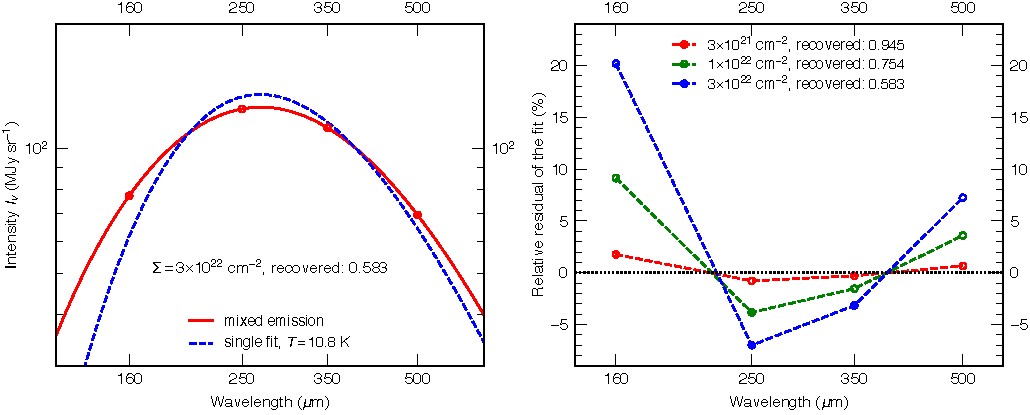
\includegraphics[width=0.96\textwidth]{fig_mixing.pdf}
\caption{\emph{Left}: the emission of a line of sight of $3{\times}10^{22}$\,cm$^{-2}$, the sum over depth of material at every
temperature, with the single modified blackbody fitted to it in the four wavebands and with the weights that the reconstruction
uses. The fit is drawn toward the warmer and brighter material, so the temperature it returns is too high and the surface density
that follows from it is too low. \emph{Right}: the relative residuals of that fit, waveband by waveband, for three total surface
densities, with the fraction of the true surface density recovered beside each. The pattern is always the same, positive at the
ends and negative in the middle, and it grows with the surface density, but it never rises above the calibration uncertainties of
$20${\%} at $160${\um} and $10${\%} at the three longer wavebands.}
\label{fig:mixing}
\end{figure*}

\subsection{Ambiguity of the fitted temperatures}
\label{app:tcorr}

The reconstruction gives a dust temperature for every pixel, together with the surface density. If the temperature of a pixel
differs from the one that the relation predicts at its surface density, the temperature carries information that the surface
density does not. Four ways of using it were tested, all calibrated on the radiative transfer models. None was adopted, and the
reason is the same for all four.

The methods were: a table of the required factor against the surface density, the fitted temperature, and the contrast between the
images at $O = 13.5$ and $36.3{\arcsec}$; a smooth function of the surface density and of the offset of the fitted temperature
from the relation, fitted to the grid of radiation fields; a table computed from analytic lines of sight through structures
embedded in a diffuse medium; and a redistribution of the correction within each beam to follow the shape of the finest image. On
the models of the subdivision grid, they changed the median core mass by $2$ to $9$\% relative to the adopted correction. The third
method under-corrected the dense material in fields of $G_0 = 20$ to $50$ by a factor of $1.5$ to $1.7$. On an earlier simulated
sky, the first two over-corrected the flanks of filaments even more than the adopted correction, and the fourth copied the noise of
the finest image into the factor.

The reason is that a warm pixel is ambiguous. A pixel can be warmer than the relation predicts for two reasons. First, a stronger
radiation field may heat it. The radiative transfer models then say that it needs more correction. Second, it may lie on the flank
of a structure, near its surface, or its line of sight may also cross a warm cloud. It then needs less correction. The models used
for the calibration contain only the first case, and the simulated sky mostly the second. A correction that uses the temperature is
therefore right in one case and wrong in the other. The fitted temperature of a single pixel cannot distinguish the two cases. The
radiation field varies over parsecs, and the warmth of a flank varies over the width of a filament. The field is therefore
estimated from the temperature of the diffuse material of the whole map, as one number for a cloud (Appendix~\ref{app:fieldest}).
In a small field, such as the Aquila field of Sect.~\ref{sec:aquila}, only $12$\% of the pixels are diffuse enough, and most of
them lie in one corner, so the field must be taken from the larger map. None of these corrections changed the core mass by more
than the error due to the background (Sect.~\ref{sec:valgrid}), so the simplest one was adopted.

\section{Uncertainties and limitations}
\label{sec:limits}

Table~\ref{tab:accuracy} collects the accuracies measured on the models of this paper, before and after the correction. The
subsections that follow discuss each source of error.

\subsection{Summary of the accuracy}
\label{sec:accuracy}

\begin{table*}[ht!]
%%%%% -----------------------------------------------------------------------------------------------------------------------------
%%%%% NUMBERS (2026-10-20): the values of this table are copied from Sects. 5, 6 and 7 and Appendices B and D; see comments there.
%%%%% -----------------------------------------------------------------------------------------------------------------------------
\caption{Accuracy of surface densities and masses derived from \emph{Herschel} images at $160$--$500${\um}, measured
on the radiative transfer models of this paper. Accuracy ratios (measured over true values) and relative errors are medians over
the models, with the 16th and 84th percentiles in parentheses where they are available; ranges span the models listed. For the
diffuse cloud, the range is that between $10^{22}$ and $10^{21}$\,cm$^{-2}$. Uncorrected: the reconstruction of \emph{hires} at
$O = 13.5{\arcsec}$, or a single modified blackbody fit. Corrected: the same after the correction of Eq.~(\ref{eq:correction}).}
\label{tab:accuracy}
\centering
\setlength{\tabcolsep}{4pt}
\begin{tabular}{llll}
\hline\hline
\noalign{\smallskip}
Quantity & Uncorrected & Corrected & Models (Section) \\
\noalign{\smallskip}
\hline
\noalign{\smallskip}
diffuse cloud, accuracy ratio of $\Sigma$               & 0.76                 & 0.89 (0.86--0.94)  & cloud model (\ref{sec:sim}) \\
total $\Sigma$ within core footprints, accuracy ratio   & 0.78 (0.56--0.93)    & 0.99 (0.92--1.03)  & 1815 cores (\ref{sec:valgrid}) \\
core mass from the image, accuracy ratio                & 0.63 (0.46--0.86)    & 0.98 (0.75--1.11)  & 1750 cores (\ref{sec:valgrid}) \\
core center ($3{\arcsec}$), relative error of $\Sigma$  & $-0.44$              & $-0.12$            & 1815 cores (\ref{sec:valgrid}) \\
filament crest, accuracy ratio of $\Sigma$              & 0.42--0.86           & 0.78--0.94         & 7 filaments (\ref{sec:cyl}) \\
filament linear density $\Lambda$, accuracy ratio       & 0.60--0.96           & 0.93--1.01         & 7 filaments (\ref{sec:cyl}) \\
filament width $H$ ($40{\arcsec}$), accuracy ratio      & 1.21--1.65           & 1.15--1.31         & 6 filaments (\ref{sec:cyl}) \\
filament slope $\alpha$, error                          & up to $-0.22$        & within $\pm 0.05$  & 7 filaments (\ref{sec:cyl}) \\
superposed structures, relative error of $\Sigma$       & --                   & $-0.13$ to $+0.21$ & analytic (\ref{app:twocomp}) \\
filament flanks in a dense cloud, relative error        & --                   & $+0.10$ to $+0.19$ & simulated sky (\ref{sec:sim}) \\
inclined layers, random, mean relative error            & --                   & $0$ to $+0.23$     & analytic (\ref{sec:incl}) \\
inclined filaments, random, mean relative error         & --                   & $0$ to $+0.08$     & analytic (\ref{sec:incl}) \\
field $G_0 = 1$ to 483 without $g$, relative error      & --                   & $-0.23$ to $+0.26$ & 9 radiation fields (\ref{sec:field}) \\
field $G_0 = 1$ to 483 with $g$, relative error         & --                   & $-0.16$ to $+0.02$ & 9 radiation fields (\ref{sec:field}) \\
local field wrong by a factor of 2.2, relative error    & --                   & $-0.10$ to $+0.13$ & 9 radiation fields (\ref{sec:field}) \\
floor $T_{\rm min}$ wrong by $\pm 1$\,K, relative error & --                   & $-0.22$ to $+0.51$ & relation (\ref{sec:floor}) \\
calibration error of 10\% at 500{\um}, $\Sigma$         & 0.16--0.18           & 0.16--0.23         & uniform bodies (\ref{sec:calerr}) \\
\noalign{\smallskip}
\hline
\end{tabular}
\end{table*}

The numbers of Table~\ref{tab:accuracy} rest on noiseless models, on the simplest backgrounds, and on the dust and the radiation
field of the models. For observers, they can be combined into a realistic total, adding the terms in quadrature. In diffuse
material, the terms are the bias that the correction leaves ($10$\%), the superposition of structures ($10$\%), a local field that
differs from the field of the cloud by a factor of about two ($10$\%), the calibration uncertainty of \emph{Herschel} of $10$\% per
waveband ($17$\%, Appendix~\ref{sec:calerr}), and an error of $1$\,K in the floor temperature $T_{\rm min}$ ($10$\%). In dense
structures, the same terms are $15$ to $20$, $15$, $15$, $20$ and $35$\%. The floor depends on the dust properties, which are not
known in a real cloud, and it is the largest term in dense structures (Appendix~\ref{sec:floor}). The total is about $30$\% in
diffuse material and about $50$\% in dense structures. In addition, the absolute dust opacity is uncertain by a factor of about
$1.5$ to $2$ \citep{Roy+2014}, and it may increase in dense cores \citep{Ossenkopf+Henning1994, Juvela+2015}. The opacity scales
all surface densities together, apart from such an increase, and no correction of the temperature bias can reduce its uncertainty.
Uncorrected images have the calibration and opacity uncertainties as well, but they are also biased: they underestimate $\Sigma$ by
$10$ to $25$\% in diffuse material and by factors of $1.3$ to $2.4$ in dense structures. The corrected temperature follows from the
corrected $\Sigma$ through the intensity at $500${\um} (Sect.~\ref{sec:aquila}), independently of the absolute opacity. By
Eq.~(\ref{eq:sensitivity}), an error of $30$ to $50$\% in $\Sigma$ corresponds to about $2$\,K at $11$ to $17$\,K. The fitted
temperatures, in contrast, are too high by $1$ to $4$\,K in dense structures. These estimates hold for fields within the grid of
models and for lines of sight without internal heating. Inclined layers and filaments can be over-corrected by a further $10$ to
$25$\% between $3.2{\times}10^{21}$ and $10^{22}$\,cm$^{-2}$ (Appendix~\ref{sec:incl}). For the mass of a core, the errors of its
footprint and background must be added (Sect.~\ref{sec:valgrid}).

\subsection{Uncertainty of the radiation field}
\label{sec:field}

%%%%% -----------------------------------------------------------------------------------------------------------------------------
%%%%% NUMBERS (2026-10-20): from Table tab:fieldR (see the comment there).
%%%%% -----------------------------------------------------------------------------------------------------------------------------
The factor $f$ was calibrated for $G_0 = 10$. In the nine fields of the grid, from $G_0 = 0.98$ to $483$, the correction without
the field factor $g$ errs by up to $+26$\% in weak fields and by up to $-23$\% for $G_0 \approx 20$--$100$ (Appendix~\ref{app:field}).
With $g$, the errors are between $-16$ and $+2$\%, within $4$\% of those at $G_0 = 10$. With $g$ built without the field being
tested, they are within $6$\% of those at $G_0 = 10$ (Table~\ref{tab:fieldR}).

The uncertainty of the field of a cloud, estimated from the spread of the temperatures of its diffuse material
(Appendix~\ref{app:fieldest}), changes the field factor by $\pm 3$\% in Aquila. A local field that differs from the field of the
cloud by a factor of $2.2$, one step of the grid, changes the corrected $\Sigma$ by $-11$ to $+11$\%, and a factor of $4.7$ by
$-19$ to $+23$\% (Table~\ref{tab:fieldR}, first column).

\subsection{Inclined layers and filaments}
\label{sec:incl}

%%%%% -----------------------------------------------------------------------------------------------------------------------------
%%%%% NUMBERS (2026-10-20): from python/paper_numbers/inclination_errors.py (the adopted factor of hicorrect2.py, G_0 = 10).
%%%%% -----------------------------------------------------------------------------------------------------------------------------
The factor was computed for lines of sight normal to a layer or perpendicular to the axis of a filament. Seen at an angle $i$ from
that direction, a layer or a filament has the same temperature profile along the line of sight, but its surface density and its
fitted surface density are both larger by the factor $1/\cos i$. The factor that it requires does not change, whereas the
correction applies the factor of a denser structure. With the adopted factor, the corrected $\Sigma$ is too high by $2$, $5$, $13$,
and $27$\% at $i = 30$, $45$, $60$, and $70\degr$ for $\Sigma_{\rm F} = 3.16{\times}10^{21}$\,cm$^{-2}$, and by $5$, $11$, $20$,
and $26$\% for $10^{22}$\,cm$^{-2}$. Below $10^{21}$\,cm$^{-2}$ the error is a few percent at most, and above
$3.2{\times}10^{22}$\,cm$^{-2}$ it vanishes, because the factor is held at its maximum there. For random orientations, the mean
error is up to $23$\% for layers and up to $8$\% for filaments, in both cases between $3.2{\times}10^{21}$ and
$10^{22}$\,cm$^{-2}$, where the factor rises most steeply.

\subsection{Floor temperature of shielded dust}
\label{sec:floor}

The size of the correction depends on Eq.~(\ref{eq:law}), and in particular on the temperature $T_{\rm min} = 7.0$\,K that dust
approaches when it is completely shielded. The factor is very sensitive to $T_{\rm min}$. Lowering $T_{\rm min}$ by $1$\,K raises
the factor by $30$\% at $10^{22}$\,cm$^{-2}$ and by $51$\% at $3{\times}10^{22}$\,cm$^{-2}$. Raising $T_{\rm min}$ by $1$\,K lowers
the factor by $13$ and $22$\%, respectively. The floor is therefore the part of the relation that most needs to be right. The fit
to $2086$ spheres and seven cylinders constrains it well (Fig.~\ref{fig:shielding}). Above $10^{23}$\,cm$^{-2}$, the models contain
too little mass to constrain the relation. Other radiative transfer models of prestellar cores also give central temperatures of
about $7$ to $8$\,K in the local radiation field \citep{Evans+2001, Zucconi+2001}. A floor of $10$\,K, as is sometimes assumed,
would substantially lower the factor at the highest surface densities. The geometry adds at most $5$\% (Sect.~\ref{sec:orient}).

\subsection{Noise and calibration errors}
\label{sec:calerr}

The correction is insensitive to noise, because it evaluates a smooth function of an image and fits nothing. Gaussian noise of
$1.5$, $0.50$, $0.30$, and $0.15$\,MJy\,sr$^{-1}$ at $160$, $250$, $350$, and $500${\um} was added to the models, and the total
corrected surface density changed by less than $0.5$\%. The amplification of the photometric errors by $7$ to $9$ found
in Appendix~\ref{app:colors} does not apply to the correction, because the underestimation is not derived from the colors. A
calibration error changes the fitted surface density $\Sigma_{\rm F}$, and the corrected surface density $f(\Sigma_{\rm
F})\,\Sigma_{\rm F}$ follows. The effect of an error of $10$\% in each waveband was computed for uniform lines of sight of
$3{\times}10^{21}$ to $10^{23}$\,cm$^{-2}$. An error at $500${\um}, the reference waveband, changes the uncorrected surface density
by $16$ to $18$\% and the corrected one by $16$ to $23$\%. An error at $160$, $250$ or $350${\um} changes the fitted temperature by
up to $0.4$\,K. It changes the uncorrected surface density by $1$ to $12$\% and the corrected one by $1$ to $11$\%. An error of
$10$\% in all wavebands at once changes the uncorrected surface density by $10$\% and the corrected one by $9$ to $13$\%. Where $f$
rises steeply with $\Sigma_{\rm F}$, between $10^{22}$ and $3{\times}10^{22}$\,cm$^{-2}$, the correction enlarges the error of the
uncorrected image by up to $1.4$ times. Where $f$ declines, at the highest surface densities, it reduces the error slightly.

\subsection{Internally heated sources}
\label{sec:notdo}

The correction assumes that the dust is heated from outside, as in the models. A line of sight through a protostar contains an
internal source, and its temperature gradient is reversed. The models do not describe such a line of sight, and the accuracy of the
correction there is unknown. Every pixel was nevertheless corrected in the same way. Leaving the protostars uncorrected would
require detecting them first, and the correction would then depend on a source extraction. The masses of protostellar cores
measured in corrected images should therefore be used with caution.

\end{document}
